%%**************************************************************
%% Vorlage fuer Bachelorarbeiten (o.ä.) der DHBW
%%
%% Autor: Tobias Dreher, Yves Fischer
%% Datum: 06.07.2011
%%
%% Autor: Michael Gruben
%% Datum: 15.05.2013
%%
%% Autor: Markus Barthel
%% Datum: 22.08.2014
%%**************************************************************

%!TEX root = ../dokumentation.tex

%
% Nahezu alle Einstellungen koennen hier getaetigt werden
%

\documentclass[%
	pdftex,
	oneside,		% Einseitiger Druck.
	12pt,			% Schriftgroesse
	parskip=half,	% Halbe Zeile Abstand zwischen Absätzen.
	headsepline,	% Linie nach Kopfzeile.
	footsepline,	% Linie vor Fusszeile.
	abstracton,	    % Abstract Überschriften
	ngerman,		% Translator
]{scrreprt}

%Seitengroesse
\usepackage{fullpage}

%Zeilenumbruch und mehr
\usepackage[activate]{microtype}

% Zeichencodierung
\usepackage[utf8]{inputenc}
\usepackage[T1]{fontenc}

% Zeilenabstand
\usepackage[onehalfspacing]{setspace}

% Index-Erstellung
\usepackage{makeidx}

% Lokalisierung (neue deutsche Rechtschreibung)
\usepackage[ngerman]{babel}

% Anführungszeichen 
\usepackage[babel,german=quotes]{csquotes}
%\usepackage[style=swiss]{csquotes}


% Spezielle Tabellenform fuer Deckblatt
\usepackage{longtable}
\setlength{\tabcolsep}{10pt} %Abstand zwischen Spalten
\renewcommand{\arraystretch}{1.5} %Zeilenabstand

% Grafiken
\usepackage{graphicx}

% Mathematische Textsaetze
%\usepackage{amsmath}
%\usepackage{amssymb}

% Pakete um Textteile drehen zu können, oder eine Seite Querformat anzeigen kann.
%\usepackage{rotating}
%\usepackage{lscape}

% Farben
\usepackage{color}
\definecolor{LinkColor}{rgb}{0,0,0.2}
\definecolor{ListingBackground}{rgb}{0.92,0.92,0.92}

\newcommand{\pdftitel}{Positionsbestimmung mit Ultraschall}
\newcommand{\autor}{Marina Del Corvo, Olaf Vogt, Christian Buss}
\newcommand{\arbeit}{Studienarbeit}

% Titel, Autor und Datum
\title{\titel}
\author{\autor}
\date{\datum}

% PDF Einstellungen
\usepackage[%
	pdftitle={\pdftitel},
	pdfauthor={\autor},
	pdfsubject={\arbeit},
	pdfcreator={pdflatex, LaTeX with KOMA-Script},
	pdfpagemode=UseOutlines, % Beim Oeffnen Inhaltsverzeichnis anzeigen
	pdfdisplaydoctitle=true, % Dokumenttitel statt Dateiname anzeigen.
	pdflang=de % Sprache des Dokuments.
]{hyperref} 

% (Farb-)einstellungen für die Links im PDF
\hypersetup{%
	colorlinks=true, % Aktivieren von farbigen Links im Dokument
	linkcolor=LinkColor, % Farbe festlegen
	citecolor=LinkColor,
	filecolor=LinkColor,
	menucolor=LinkColor,
	urlcolor=LinkColor,
	bookmarksnumbered=true % Überschriftsnummerierung im PDF Inhalt anzeigen.
}

% Literaturverweise (mit deutschem und)
\usepackage[
	    backend=biber,      % empfohlen. Falls biber nicht installierbar: bibtex
	    bibwarn=true,
	    bibencoding=utf8, 	% wenn .bib in utf8, sonst ascii
	    sortlocale=de_DE,
	    style=alphabetic 	%Zitierstil. Siehe http://ctan.mirrorcatalogs.com/macros/latex/contrib/biblatex/doc/biblatex.pdf 
]{biblatex}
\addbibresource{ArbeitBib.bib}

% Verschiedene Schriftarten
%\usepackage{goudysans}
%\usepackage{lmodern}
%\usepackage{libertine}
\usepackage{palatino} 

% Hurenkinder und Schusterjungen verhindern
% http://projekte.dante.de/DanteFAQ/Silbentrennung
\clubpenalty=10000
\widowpenalty=10000
\displaywidowpenalty=10000

% Quellcode
\usepackage{listings}
\lstloadlanguages{Python}
\lstset{%
	language=Python,		 	 % Sprache des Quellcodes
	%numbers=left,           % Zelennummern links
	stepnumber=1,            % Jede Zeile nummerieren.
	numbersep=5pt,           % 5pt Abstand zum Quellcode
	numberstyle=\tiny,       % Zeichengrösse 'tiny' für die Nummern.
	breaklines=true,         % Zeilen umbrechen wenn notwendig.
	breakautoindent=true,    % Nach dem Zeilenumbruch Zeile einrücken.
	postbreak=\space,        % Bei Leerzeichen umbrechen.
	tabsize=2,               % Tabulatorgrösse 2
	basicstyle=\ttfamily\footnotesize, % Nichtproportionale Schrift, klein für den Quellcode
	showspaces=false,        % Leerzeichen nicht anzeigen.
	showstringspaces=false,  % Leerzeichen auch in Strings ('') nicht anzeigen.
	extendedchars=true,      % Alle Zeichen vom Latin1 Zeichensatz anzeigen.
	captionpos=b,            % sets the caption-position to bottom
	backgroundcolor=\color{ListingBackground} % Hintergrundfarbe des Quellcodes setzen.
}

% Glossar
\usepackage[
	nonumberlist, %keine Seitenzahlen anzeigen
	%acronym,      %ein Abkürzungsverzeichnis erstellen
	%section,     %im Inhaltsverzeichnis auf section-Ebene erscheinen
	toc,          %Einträge im Inhaltsverzeichnis
]{glossaries}

%Akronyme
\usepackage[printonlyused,footnote]{acronym}

% Fussnoten
\usepackage[perpage, hang, multiple, stable]{footmisc}

%Bildpfad
\graphicspath{{images/}}

%nur ein latex-Durchlauf für die Aktualisierung von Verzeichnissen nötig
\usepackage{bookmark}

%Gleitumgebungen (Bilder, Tabellen, usw\ldots) lassen sich mit H an genau der
% definierten Stelle platzieren
\usepackage{float}

% für die vertikale Platzierung von Text in Tabellen
\usepackage{array}

% für die Darstellung des Euro-Symbols
\usepackage[right]{eurosym}

% für textumflossene Grafiken
\usepackage{wrapfig}

% eine Kommentarumgebung "k" (Handhabe mit \begin{k}<Kommentartext>\end{k},
% Kommentare werden rot gedruckt). Wird \% vor excludecomment{k} entfernt,
% werden keine Kommentare mehr gedruckt.
\usepackage{comment}
\specialcomment{k}{\begingroup\color{red}}{\endgroup}
%\excludecomment{k}


\makeglossaries
%!TEX root = ../dokumentation.tex

%
% vorher in Konsole folgendes aufrufen: 
%	makeglossaries makeglossaries dokumentation.acn && makeglossaries dokumentation.glo
%

%
% Glossareintraege --> referenz, name, beschreibung
% Aufruf mit \gls{...}
%
\newglossaryentry{Glossareintrag}{name={Glossareintrag},plural={Glossareinträge},description={Ein Glossar beschreibt verschiedenste Dinge in kurzen Worten}}


\begin{document}

	% Deckblatt
	\begin{spacing}{1}
		%!TEX root = ../dokumentation.tex

\begin{titlepage}
	\begin{longtable}{p{8.2cm} p{5.4cm}}
%		{\raisebox{\ht\strutbox-\totalheight}{\includegraphics{images/firma-deckblatt.png}}} &
		{\raisebox{\ht\strutbox-\totalheight}{
\includegraphics[height=2.5cm]{images/dhbw.png}}}
	\end{longtable}
	\enlargethispage{20mm}
	\begin{center}
		\vspace*{12mm}	{\LARGE\bf \titel }\\
		\vspace*{12mm}	{\large\bf \arbeit}\\
		\vspace*{12mm}	\langdeckblattabschlusshinleitung\\
		\vspace*{3mm}		{\bf \abschluss}\\
    \vspace*{12mm}	\langartikelstudiengang{} \studiengang\\
    \vspace*{3mm}		\langanderdh{} \dhbw\\
		\vspace*{12mm}	\langvon\\
		\vspace*{3mm}		{\large\bf \autor}\\
		\vspace*{12mm}	\datumAbgabe\\
	\end{center}
	\vfill
	\begin{spacing}{1.2}
	\begin{tabbing}
		mmmmmmmmmmmmmmmmmmmmmmmmmm             \= \kill
%		\textbf{\langdbbearbeitungszeit}       \>  \zeitraum\\
		\textbf{\langdbkurs}  \>  \kurs\\
%		\textbf{\langdbfirma}                  \>  \firma, \firmenort\\
		\textbf{\langdbgutachter, \langdbbetreuer}               \>  \betreuer\\
%		\textbf{\langdbgutachter}              \>  \gutachter
	\end{tabbing}
	\end{spacing}
\end{titlepage}

	\end{spacing}
	\newpage

	\renewcommand{\thepage}{\Roman{page}}
	\setcounter{page}{1}

	% Sperrvermerk
%	%!TEX root = ../dokumentation.tex

\thispagestyle{empty}
% Sperrvermerk direkt hinter Titelseite
\section*{\langsperrvermerk}

\vspace*{2em}

\iflang{de}{%
  Die vorliegende {\arbeit} mit dem Titel {\itshape{} \titel{}\/} ist mit einem Sperrvermerk versehen und wird ausschließlich zu Prüfungszwecken am Studiengang {\studiengang} der Dualen Hochschule Baden-Württemberg {\abgabeort} vorgelegt.
Jede Einsichtnahme und Veröffentlichung – auch von Teilen der Arbeit – bedarf der vorherigen Zustimmung durch die {\firma}.
}
\iflang{en}{%
%http://www.ib.dhbw-mannheim.de/fileadmin/ms/bwl-ib/Downloads_alt/Leitfaden_31.05.pdf
  The {\arbeit} on hand {\itshape{} \title{}\/} \langanderdh{} {\abgabeort} contains internal resp.\ confidential data of {\firma}. It is strictly forbidden, to distribute the content of this paper (including data, figures, tables, charts etc.) as a whole or in extracts, to make copies or transcripts of this paper or of parts of it, to display this paper or make it available in digital, electronic or virtual form.
Exceptional cases may be considered through permission granted in written form by the author and {\firma}.
}

%	\newpage

	% Erklärung
	%!TEX root = ../dokumentation.tex

\thispagestyle{empty}

\section*{\langerklaerung}
% http://www.se.dhbw-mannheim.de/fileadmin/ms/wi/dl_swm/dhbw-ma-wi-organisation-bewertung-bachelorarbeit-v2-00.pdf
\vspace*{2em}

\iflang{de}{%
Ich erkläre hiermit ehrenwörtlich: \\
\begin{enumerate}
\item dass ich meine {\arbeit} mit dem Thema
{\itshape \titel } ohne fremde Hilfe angefertigt habe;
\item dass ich die Übernahme wörtlicher Zitate aus der Literatur sowie die Verwendung der Gedanken
anderer Autoren an den entsprechenden Stellen innerhalb der Arbeit gekennzeichnet habe;
\item dass ich meine {\arbeit} bei keiner anderen Prüfung vorgelegt habe;
\item dass die eingereichte elektronische Fassung exakt mit der eingereichten schriftlichen Fassung
übereinstimmt.
\end{enumerate}

Ich bin mir bewusst, dass eine falsche Erklärung rechtliche Folgen haben wird.
}

\iflang{en}{%
Unless otherwise indicated in the text or references, or acknowledged
above, this thesis is entirely the product of my own scholarly work. This
thesis has not been submitted either in whole or part, for a degree at this
or any other university or institution. This is to certify that the printed
version is equivalent to the submitted electronic one.
}

\vspace{3em}

\abgabeort, \datumAbgabe
\vspace{4em}

\autor

	\newpage

	% Abstract
%	%!TEX root = ../dokumentation.tex

\pagestyle{empty}

\renewcommand{\abstractname}{Zusammenfassung}
\begin{abstract}
Ein Abstract ist eine prägnante Inhaltsangabe, ein Abriss ohne
Interpretation und Wertung einer wissenschaftlichen Arbeit. In DIN
1426 wird das (oder auch der) Abstract als Kurzreferat zur
Inhaltsangabe beschrieben.

\begin{description}
\item[Objektivität] soll sich jeder persönlichen Wertung enthalten
\item[Kürze] soll so kurz wie möglich sein
\item[Genauigkeit] soll genau die Inhalte und die Meinung der Originalarbeit wiedergeben
\end{description}

Üblicherweise müssen wissenschaftliche Artikel einen Abstract
enthalten, typischerweise von 100-150 Wörtern, ohne Bilder und
Literaturzitate und in einem Absatz.

Quelle \url{http://de.wikipedia.org/wiki/Abstract} Abgerufen 07.07.2011
\end{abstract}




%	\newpage

	\pagestyle{plain}

	% Inhaltsverzeichnis
	\begin{spacing}{1.1}
		\setcounter{tocdepth}{1}
		%für die Anzeige von Unterkapiteln im Inhaltsverzeichnis
		%\setcounter{tocdepth}{2}
		\tableofcontents
	\end{spacing}
	\newpage

	\renewcommand{\thepage}{\arabic{page}}
	\setcounter{page}{1}

	% Inhalt
	%!TEX root = ../dokumentation.tex

\chapter{Projekteinführung}
Die vorliegende Arbeit handelt von der Positionsbestimmung mittels Ultraschall, wie sie z.B. auch bereits für die Abstandsmessungen bei PKWs (Einparkhilfen) eingesetzt wird. Dabei gibt es zwei unterschiedliche Methoden, um die Abstände zwischen zwei oder mehr Gegenständen zu ermitteln. Entweder führt man eine direkte oder eine indirekte Messung durch. Für eine direkte Messung ist es nötig, dass die Position zweier Punkte, deren Abstand man messen möchte, bekannt ist. Dann wird eine unmittelbare Abstandsmessung mit Hilfe eines Maßstabes (z.B. Zentimeter) durchgeführt, um den Abstand zwischen den beiden Punkten zu bestimmen. Um allerdings unabhängig von der Position den Abstand ermitteln zu können, bedarf es einer indirekten Abstandsmessung. Diese erfolgt indem nicht die Entfernung direkt, sondern eine von ihr abhängige Größe ( die Signallaufzeit) gemessen wird. Im Folgenden Versuchsaufbau soll die Position eines Gegenstands ermittelt werden, welcher sich im Wellenkegel dreier Ultraschallsender bzw. Empfänger befindet. Bevor jedoch die eigentliche Messung gestartet wird, ermittelt man zunächst die relative Position der Sender-Empfänger-Konstruktionen im Raum, indem einer der Sender ein Ultraschallsignal aussendet, welches von den Empfängern der  jeweils anderen Sender-Empfänger-Konstruktionen empfangen wird. Über die bereits erwähnte Signallaufzeit, lässt sich der Abstand zwischen den beiden Sender-Empfänger-Konstruktionen messen. Mittels Trilateration kann so die genaue Position der drei Sender-Empfänger-Konstruktionen ermittelt werden. Nach dem selben Prinzip wird dann letzten Endes auch die Position und der Abstand zum Gegenstand in deren Mitte bestimmt.\\
Die vorliegende Arbeit enthält die theoretischen Grundlagen, die notwendigen Konstruktionsanleitungen der entwickelten und genutzten Bauteile, sowie die Beschreibung der Oberfläche für die Darstellung der Messergebnisse. Außerdem noch die wichtigsten Problembehandlungen, sowie die notwendige Schnittstellenkommunikation.


\section{Ultraschall Grundlagen}
Bevor der genaue Vorgang bei der Positionsbestimmung mittels Ultraschalls beschrieben wird, sollen hier zunächst einige Grundlagen und Kenntnisse über den Ultraschall im Allgemeinen zum besseren Verständnis beitragen:
\subsection{Was genau ist Ultraschall?}
Bei Ultraschall handelt es sich um Schallfrequenzen, oberhalb des hörbaren Frequenzbereichs des Menschen. Diese Aussage zu präzisieren ist allerdings schwierig, denn dieser Bereich unterliegt individuellen Wahrnehmungsschwankungen und um-fasst daher Frequenzen ab etwa 16 kHz.\footnote{nach DIN 1320 Akustik Begriffe} Bei Frequenzen unterhalb des für Menschen hörbaren Bereichs handelt es sich um Infraschall. Ab einer Schallfrequenz von etwa $1GHz$ spricht man von Hyperschall. 
\begin{figure}[H]
	\centering
	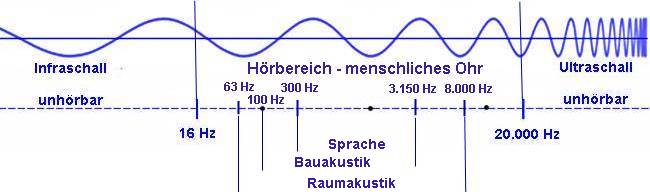
\includegraphics[scale=0.9]{images/hoerbarer_Schall-Infraschall-Ultraschall.jpg}
	\caption{Frequenzbereich des Schalls\footnotemark}
\end{figure}
\footnotetext{\url{http://www.haustechnikdialog.de/SHKwissen/Images/hoerbarer\_Schall-Infraschall-Ultraschall.jpg}}


\subsection{Wie breitet sich Ultraschall aus?}
Die Ausbreitung der Ultraschallwellen hängt von der Beschaffenheit des zu durch-dringenden Mediums ab: Im Innern von Gasen und Flüssigkeiten breitet sich Ultraschall überwiegend als Longitudinalwelle (Längswellen - Schwingungsrichtung der einzelnen Oszillatoren ist parallel zur Ausbreitungsrichtung der Welle) aus. In Festkörpern kommt es jedoch zu Schubspannungen die dazu führen, dass die Ultraschallwellen sich zusätzlich in Transversalwellen (Schwingungsrichtung der einzelnen Oszillatoren ist orthogonal zur Ausbreitungsrichtung der Welle) ausbreiten.
Prinzipiell erfährt die Schallwelle bei der Ausbreitung einen Verlust an Schallintensität und der damit verbundenen Schallfeldgrößen. Diese werden beim Durchdringen eines Mediums durch Absorption, Reflexion, Brechung, Streuung und Schallfeldgeometrie abgeschwächt. Ursachen für die Absorption sind: innere Reibung, Wärmeleitung und Relaxationen. Die Absorption führt dazu, dass die Schallwellenreichweite begrenzt ist und die Frequenz an die Eindringtiefe angepasst werden muss. Luft weist eine stark mit der Frequenz steigende Dämpfung für Ultraschall auf, was für den späteren Versuchsaufbau dieser Arbeit von Bedeutung sein wird. \\
Der Zusammenhang zwischen der Frequenz $\nu $ und der Wellenlänge $\lambda$ der Schallwelle ist formal derselbe wie beim Licht, allerdings mit anderer Ausbreitungsgeschwindigkeit fehlender Dispersion:
\begin{equation}
c=\lambda*\nu
\end{equation}
Weil es sich bei Schallwellen um longitudinale Materie-Wellen handelt können diese sich auch nicht in einem Vakuum ausbreiten (physikalisch gesehen ist Schall eine als Welle fortschreitende mechanische Deformation in einem Medium und braucht daher immer ein Trägermedium, z.B. Luft). 


\section{Indirekte Abstandsmessung durch Laufzeitmessung}
Das Prinzip, welches hinter einer Abstandsbestimmung mittels Laufzeitmessung steckt, entspricht dem eines Echos. Wegen der zugrundeliegenden, physikalischen Eigenschaft mancher Materialien den Schall zu reflektieren kann daraus eine Methode zur Abstandsbestimmung abgeleitet werden. Ein Schallimpuls (Rufen) wird losgeschickt, am Hindernis reflektiert und die Zeit bis zu seiner Rückkehr (Echo) zur Schallquelle gemessen. Anhand der bekannten Ausbreitungsgeschwindigkeit des Schalls in Luft lässt sich die Entfernung zum Hindernis berechnen.


\begin{figure}[H]
	\centering
	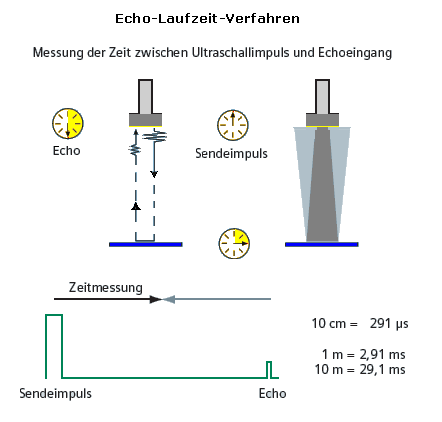
\includegraphics[scale=0.8]{images/Echo-Laufzeit-Verfahren.png}
	\caption{Echo-Laufzeit-Verfahren\footnotemark}
\end{figure}
\footnotetext{\url{https://de.wikipedia.org/wiki/Ultraschall}}

Bei Laufzeitmessungen werden im Wesentlichen nur Zeitdifferenzen bestimmt. Daher benötigt man- im Gegensatz zu Messungen in einer absoluten Zeitskala (Weltzeit, Atomzeit usw.)- nur ein relatives Zeitsystem, also ohne definierten Nullpunkt.

\subsection{Das Echosignal}
Ein Echosignal setzt sich aus verschiedenen Signalanteilen zusammen:
\begin{figure}[H]
	\centering
	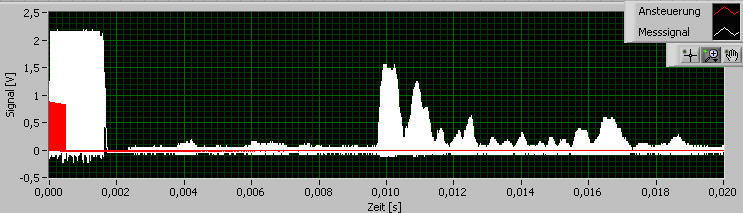
\includegraphics[scale=0.6]{images/echosignal.png}
	\caption{Aufnahme eines Echosignals\footnotemark}
\end{figure}
\footnotetext{\url{http://tu-dresden.de/die\_tu\_dresden/fakultaeten/fakultaet\_elektrotechnik\_und\_informationstechnik/iee/mst/studium/lehre/MST/dl/Pr/us}}

Ganz vorne links ist der gesendete Ultraschallimpuls zu sehen. Dieser Puls ist bereits auffallend länger als das tatsächliche Ansteuersignal. Der Grund hierfür ist das lange Ausschwingen des Ultraschallwandlers und die Verstärkerelektronik. Infolge dessen kann es zu einer Überlagerung des ausschwingenden Sendepulses mit dem ersten Echosignal kommen was wiederum zu einer Begrenzung des minimal messbaren Abstands führt.\\
Weiter rechts in der Abbildung sind die eigentlichen Reflexionen des Ultraschallpulses zu sehen, gefolgt von weiteren Überlagerungen, die durch unmittelbare Reflexion des Hindernisses als auch aus Mehrfachreflexionen bestehen. Diese Mehrfachreflexion ist die fortlaufende Reflexion eines früheren Ultraschallpulses zwischen dem Hindernis und der Messvorichtung. Dieser Hin- und herlaufende Ultraschallpuls wird zwar zunehmend gedämpft, wird jedoch trotzdem mit kleinerer Amplitude in den nachfolgenden Echosignalen sichtbar bleiben.\\
Das Auftreten dieser Mehrfachreflexionen führt zu einem komplexen Aussehen des zu deutenden Echosignals und erschwert die Erkennung des eigentlichen Echos des Hindernisses. Daher muss die Erkennung mit Hilfe eines Schwellwertes erfolgen, welcher jedoch für eine begrenzte Verlässlichkeit der Abstandsmessung sorgt.

\subsection{Ultraschallsender}
Um Ultraschall zu erzeugen eignen sich dynamische und elektrostatische Lautsprecher, sowie insbesondere Piezolautsprecher.  Bei letzterem handelt es sich um Membran-gekoppelte Platten aus piezoelektrischer Keramik, die durch Umkehr des Piezo-Effekts\footnote{Änderung der elektrischen Polarisation und somit das Auftreten einer elektrischen Spannung an Festkörpern, wenn sie elastisch verformt werden} zu Schwingungen angeregt werden. Mit Hilfe von piezoelektrischer Kunststoffe (PVDF) lassen sich auch direkt Membranen ansteuern, was ein verbessertes Übertragungsverhalten hervorruft.

\subsection{Ultraschallempfänger}
Der Empfang von Ultraschallwellen kann prinzipiell mit den gleichen elektrischen Wandlern erfolgen, wie sie auch zu dessen Erzeugung verwendet werden. Die so erhaltenen elektrischen Signale können einer Frequenz-, Phasen- oder Amplitudenauswertung unterzogen werden.

\section{Positionsbestimmung}
Für die Positionsbestimmung eines Gegenstands, welcher sich zwischen drei Ultraschallsensoren befindet muss zunächst die genaue Position der Sensoren festgelegt, bzw. ermittelt werden. Dies erfolgt ebenfalls über eine Abstandsmessung: 
Abwechselnd senden die Sender einen Ultraschallimpuls, und ermitteln mittels eines direkt daneben angebrachten Empfängers den Abstand zum nächsten Sensor. Da nicht alle Sensoren exakt gleich gut messen werden die beiden Abstandswerte zwischen zwei Sensoren im Anschluss noch gemittelt. Direkt danach messen die Sensoren den Abstand zum Gegenstand in der Mitte bestimmen dadurch dessen genaue Position.


	%!TEX root = ../dokumentation.tex

% Kapitel als Übersicht des Projekts
% Inhalt: Zielsetzung, Entiwcklung/Umsetzung, Hardware, Architektur, Tools


\chapter{Projektübersicht}

%\section{Ziel}
Das Ziel des Projektes ist es, die Position eines Objektes mithilfe von Ultraschallsensoren zu messen. Dabei reicht die Position auf einer Fläche, sie muss daher nur zweidimensional bestimmt werden. Das Ergebnis wird anschließend auf einem Bildschirm visualisiert.\\
Da es sich dabei bereits um ein komplexes System handelt, bei dem es an vielen Stellen zu unerwarteten Problemen kommen kann, wurde ein vorrangiges Ziel definiert. Zuerst sollte eine einzelne Abstandsmessung durchgeführt und bewertet werden. Diese Aufgabe umfasst bereits alle physikalische Prinzipien, die zur Positionsbestimmung genutzt werden. Sobald die Abstandsmessung zuverlässig funktioniert, kann das endgültige System darauf aufgebaut werden.


\section{Architektur, Lösungsansatz} % Hier wird auch die Hardware beschrieben
Für die Positionsbestimmung werden drei Sender und Empfänger verwendet. Davon ist jeweils einer auf einer Platine verbaut, auf der sich zusätzlich Schaltungen für die Signalverarbeitung und ein Mikrocontroller befinden. Die drei Platinen werden so angeordnet, dass sie Objekte in ihrer Mitte erkennen können. Sie sind alle mit einem Einplatinen-Computer verbunden, mit dem die Mikrocontroller über einen \ac{TWI}-Bus kommunizieren können. Zwischen dem Computer und den Sensorplatinen befindet sich eine Verteilerplatine, an der die Stromversorgung eingesteckt wird und die Leitungen von Computer zu Platinen entsprechend verdrahtet sind. %TODO: Vertratet geeignetes Wort?
Zur Verbindung untereinander werden Flachbandkabel verwendet. Die Verteilerplatine besitzt zusätzlich einen Steckplatz mit einer Standard-\ac{ISP}-Pinbelegung, mit dem die Mikrocontroller direkt vom Einplatinen-Computer beschrieben werden können.\\
% Bild Architektursübersicht
\begin{figure}[H] %TODO: Bildschirm kann auch mit rein. Sensoren als Ellipsen darstellen.
\centering
\begin{tikzpicture}
%\filldraw[fill=black!20, draw=black] (0,0) -- (10,0) -- (10,5) -- (0,5) -- (0,0);

% Positionen der Platinen
\coordinate (s1) at (0, 0);
\coordinate (s2) at (3.3, 5.2);
\coordinate (s3) at (-3.3, 5.2);
\coordinate (com) at (-6.5, -1);
\coordinate (ver) at (-4, -1);
\coordinate (ob) at (-0.5, 3.5);

% Verbindungen
% Computer-Verteiler
\draw (com) -- (ver);
% Verteiler-Sensor1
\draw (ver) -- (0,-1);
% Verteiler-Sensor2
\draw (ver) |- (0,-1.7) -| ($(s2) + (1,0)$);
% Verteiler-Sensor3
\draw (ver) |- (s3);

% Platine 1
\begin{scope}[shift=(s1), rotate around={180:(s1)}]
	\filldraw[fill=red!60!black, draw=black] (-0.5,0) rectangle (0.5, 1.5);
	\fill[fill=black!80, draw=black] (0.1, 0) circle (0.1);
	\fill[fill=black!80, draw=black] (-0.1,0) circle (0.1);
	\node[right] at (-0.7,1) {Sensorplatine 1};
\end{scope}

% Platine 2
\begin{scope}[shift=(s2), rotate around={300:(s2)}]
	\filldraw[fill=red!60!black, draw=black] (-0.5,0) rectangle (0.5, 1.5);
	\fill[fill=black!80, draw=black] (0.1, 0) circle (0.1);
	\fill[fill=black!80, draw=black] (-0.1,0) circle (0.1);
	\node at (0, 3) {Sensorplatine 2};
\end{scope}

% Platine 3
\begin{scope}[shift=(s3), rotate around={60:(s3)}]
	\filldraw[fill=red!60!black, draw=black] (-0.5,0) rectangle (0.5, 1.5);
	\fill[fill=black!80, draw=black] (0.1, 0) circle (0.1);
	\fill[fill=black!80, draw=black] (-0.1,0) circle (0.1);
	\node at (0, 3) {Sensorplatine 3};
\end{scope}

% Objekt
\filldraw[fill=green!50, draw=black] (ob) circle (0.7);
\node at (ob) {Objekt};

% Verteilerplatine
\begin{scope}[shift=(ver)]
	\filldraw[fill=brown!70, draw=black] (-0.25, -0.5) rectangle (0.25, 0.5);
	\node[below] at (0, -0.7) {Verteilerplatine};
\end{scope}

% Raspberry PI
\begin{scope}[shift=(com)]
	\filldraw[fill=blue!70!black!70!white, draw=black] (-0.5, -0.75) rectangle (0.5, 0.75);
	\node[above] at (0, 0.75) {Computer};
\end{scope}

\end{tikzpicture}
\caption{Schema der Architektur} \label{fig:ARCH}
\end{figure}


\subsection{Sensorplatine und Mikrocontroller}
Die Mikrocontroller auf den Sensorplatinen erfüllen die Zwecke:
\begin{itemize}
	\item Ansteuerung der Ultraschallsender
	\item Signal am Empfänger detektieren
	\item Laufzeitmessung durchführen
	\item Status über \ac{LED}s anzeigen
	\item Schnittstelle nach außen über das \ac{TWI} bereitstellen
\end{itemize}
Verwendet wurde dafür der \textit{ATmega8} von Atmel.  %TODO


\subsection{Computer}
Der Einplatinen-Computer hat folgende Aufgaben:
\begin{itemize}
	\item Das Timing der Messungen kontrollieren
	\item Messergebnisse sammeln und auswerten
	\item Berechnete Position darstellen
	\item Ein \ac{GUI} bereitstellen
\end{itemize}
Für diesen Zweck wird ein \textit{Raspberry PI} verwendet. Er besitzt ein \ac{GPIO}-Interface, mit dem die Mikrocontroller gesteuert werden können, sowie ein \ac{HDMI}-Ausgang für die Visualisierung auf einem Bildschirm. Auf dem Computer läuft ein \textit{Archlinux}, dass speziell für die mobilen \textit{ARM}-Prozessoren angepasst wurde.\footnote{\url{http://archlinuxarm.org/}}



\section{Entwicklung} %TODO
Liste an Dingen, die entwickelt werden müssen, damit der Entwurf funktioniert.
Sensorplatine:
Sendeschaltung,
Empfängerschaltung,
Firmware für Mikrocontroller.

Protokoll für TWI-Bus

Ablauf und Timing der Messungen
Software auf RPI zum Ansteuern der Controller
GUI auf RPI



\section{Verwendete Tools} %TODO
Um Schaltungen zu entwerfen sind einige Programme zum Einsatz gekommen. Damit ließen sich die Funktionen überprüfen, Frequenzgänge berechnen und es konnten Platinen mit den fertigen Schaltplänen designt werden.
\begin{description}
	\item[KiCAD] ist ein open-source Programm, mit dem modulare Schaltpläne gezeichnet werden können, woraus sich anschließend CAD-Modelle einer Platine erstellen lassen. Das Programm wird maßgeblich am CERN entwickelt und unterstützt viele zusätzliche Funktionen. So kann z.B. eine Netzliste für die \ac{SPICE}-Engine erstellt werden, mit der die Schaltungen simuliert werden können.\footnote{\url{http://www.kicad-pcb.org/}}
	\item[LTspice] ist ein Tool von \textit{Linear Technology} um analoge und digitale Schaltungen zu simulieren, insbesondere mit den firmeneigenen Operationsverstärkern. Das Programm basiert auf dem Simulator \ac{SPICE} und besitzt einen eigenen Schaltungseditor.\footnote{\url{http://www.linear.com/designtools/software/\#LTspice}}
	\item[AktivFilter] ist ein Tool um Frequenzfilter mit Operationsverstärkern zu entwerfen. Aus einigen Vorgaben berechnet das Programm ein Bode-Diagramm, dimensioniert die Bauteile und stellt einen Schaltplan zur Verfügung.\footnote{\url{http://www.softwaredidaktik.de/filter/}}
\end{description}



	%!TEX root = ../dokumentation.tex

% Kapitel über Schaltungen, Signalerzeugung und -verarbeitung
\chapter{Schaltungen}


% Section über Sender-Schaltung, Signalerzeugung
\section{Sender} %TODO Sender Einleitung
Der Ultraschallsender wird durch ein $40 kHz$-Signal angeregt und erzeugt einen Schallkegel mit etwa $80^\circ$ Abstrahlwinkel. Der Schallpegel sollte dabei möglichst hoch sein, um die erfolgreiche Signalauswertung des reflektierten Signals auch über weite Distanzen und geringen Reflexionsfaktoren zu ermöglichen. Es wird empfohlen, den Sender mit einem Rechtecksignal anzusteuern. Durch sein sehr schmales Spektrum/Frequenz (FIXME) schwingt er dennoch sinusförmig ohne Oberwellen zu erzeugen und nimmt dabei am meisten Energie auf. (FIXME bei gleichbleibender Amplitude im vgl zu anderen Signalen/Sinus). Weiter mit Kapazität des Senders


\subsection{Signalerzeugung}
Das Rechtecksignal wird von dem Mikrocontroller erzeugt. Er besitzt einen Hardwarezähler, der mit einem Ausgangspin verbunden werden kann. Damit lässt sich ein präzises Signal erzeugen, ohne die Rechenleistung des Controllers einzuschränken.\\
Der Sender hat eine maximale Spitze-Spitze-Spannung von $U_{SS} = 20V$, das ausgegebene Signal des Mikrocontrollers wechselt jedoch nur zwischen $0V$ und $5V$. Die Sendeleistung wäre zu schwach, außerdem sollte der Ausgang des Mikrocontrollers nicht direkt belastet werden, da er nur sehr begrenzt Strom liefern kann. Aus diesen Gründen wurden mehrere Sendeverstärker entwickelt und untersucht, ob sie geeignet sind.



\subsection{Erste Schaltung: Verstärkung mit Operationsverstärker}
\subsubsection{Idee} % FIXME Differenzverstärker
Mithilfe eines Operationsverstärkers lassen sich einfach Spannungen verstärken. Mit der Komparatorschaltung kann das $0/5V$-Signal auf $-10/+10V$ umgesetzt werden. Gewählt wurde der Operationsverstärker \textit{LM258}, da seine Spannungsversorgung sehr hoch gewählt werden kann und er eine Bandweite von $1.1MHz$ hat, was für diese Zwecke ausreichen sollte.
\begin{figure}[H]
\centering
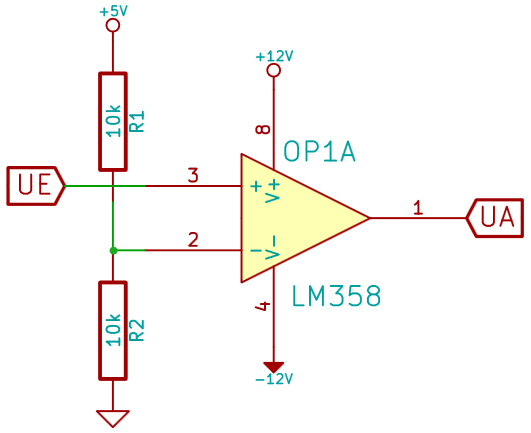
\includegraphics[scale=0.5]{images/komparatorschaltung.jpg}
\caption{Einfache Komparatorschaltung zum Umsetzen der Spannungen} \label{img:I1} %TODO: LM258/358
\end{figure}

\subsubsection{Problematik}
Bereits bei der Planung der Schaltung wurde befürchtet, dass der maximale Strom des Operationsverstärkers für ein scharfes Signal sehr knapp dimensioniert ist ($I_{Source}=30mA; I_{Sink}=40mA$). Nimmt man an, der Operationsverstärker besitzt einen Ausgangswiderstand von $0 \Omega$ und die Ladespannung beträgt $20V$, ist die Zeit zum vollständigen Laden des Senders:
\begin{equation}
t=\frac{Q}{I}=\frac{C*U}{I}=\frac{2.55nF*20V}{30mA}=1.7\mu s
\end{equation}
Im Vergleich zur Pulsdauer von $12.5\mu s$ ist dieser Wert in Ordnung. Allerdings besitzt nur ein idealer Operationsverstärker einen $0\Omega$-Ausgangswiderstand und der Sender ist auch kein idealer Kondensator. Deshalb wurde erwartet, dass die Flanken etwas abgeflacht werden.\\
Tatsächlich wurde jedoch ein viel wichtigerer Wert im Datenblatt übersehen. Die \textit{Slew Rate} gibt an, wie schnell sich die Spannung des OPs ändern kann. Beim \textit{LM258} beträgt sie $0.6V/\mu s$. Das Ausgangssignal entsprach aus diesem Grund einem Dreiecksignal und schwankte nur um wenige Volt.
% Bild von Simulation
\begin{figure}[H] %TODO: Kontrast von Bild erhöhen. Außerdem stimmen die 20V/µs nur ungefähr.
\centering
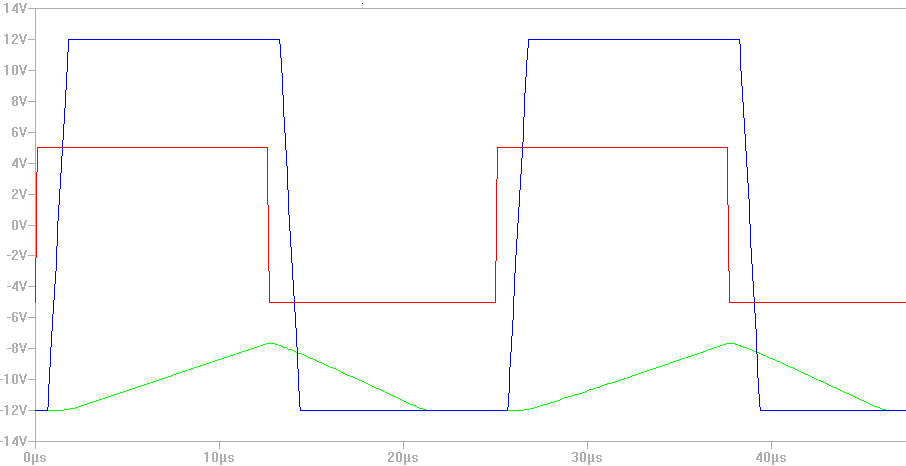
\includegraphics[scale=0.6]{images/signalverlauf_opamps.png}
\caption{Simulierter Signalverlauf von zwei Operationsverstärkern. Rot: Ansteuersignal. Grün: Slew-Rate $0.6V/\mu s$. Blau: Slew-Rate $20V/\mu s$.} \label{img:I2}
\end{figure}

\subsubsection{Fazit}
Die Spannungsverstärkung mit dem Operationsverstärker \textit{LM258} hat sich als nicht praktikabel herausgestellt, da er zu langsam reagiert. Für diese Zwecke können jedoch spezielle \textit{Komparatoren} verwendet werden, die sich wie Operationsverstärker verhalten, nur viel schneller und ungenauer sind. Die Genauigkeit spielt beim Umschalten keine Rolle.\\
Nach dieser Feststellung wurden Schaltungen mit Transistoren untersucht, da sie höhere Leistungen und schnellere Reaktionszeiten zulassen. Die Lösung mit Komparator wurde für den Fall, dass die weiteren Schaltungen keine befriedigende Ergebnisse liefern, für später aufgehoben.


\subsection{Zweite Schaltung: Verstärkung mit Transistor}
Diese Schaltung sollte möglichst einfach umsetzbar sein, da sie auch für Testzwecke verwendet werden soll. Die Spannungen sollten mit Bipolartransistoren geschaltet werden.

\subsubsection{Emitterschaltung}


\subsubsection{Spannungsbereich ausschöpfen}
Als Spannungsversorgung stehen $+5V$, $+12V$ und $-12V$ zur Verfügung. Es gibt verschiedene Schaltungen, die unterschiedliche Spannungsbereiche bieten:
\begin{description}
	\item[NPN-Transistor:] Gebräuchliche Schaltung um einen Schalter mit einen Transistor zu realisieren. Die $5V$ werden auf $12V$ verstärkt.
	\item[PNP-Transistor:] Mit nur einem Transistor kann das Signal auf $-12V$-$+5V$ umgesetzt werden. Die Spitze-Spitze-Spannung beträgt $17V$.
	\item[Zwei Transistoren:] Kombiniert man beide Verstärker, kann das Signal auf $-12V$-$+12V$ verstärkt werden. Da die Spitze-Spitze-Spannung des Senders um $4V$ überstiegen wird, muss sie mit einer Z-Diode begrenzt werden. Sie wird in Reihe entgegen der Spannung geschaltet, sodass an ihr die nötige Spannung abfällt.
	\item[Wechselsignal:] Der Sender ist nicht gegen Masse geschaltet, sondern erhält am anderen Pin das invertierte Signal. Dadurch lässt sich die Spitze-Spitze-Spannung verdoppeln. Es wird mindestens ein Transistor mehr benötigt, um die zweite Seite zu schalten. Allerdings bietet sich dafür keine Spannung an, da die $12V$ zu groß und die $5V$ zu klein sind, um die maximalen $20V$ zu erreichen.
\end{description}

%TODO: Bild

\subsubsection{Nachteile}



\subsection{Dritte Schaltung: Gegentaktausgangsstufe, Push/Pull}

\subsubsection{Idee}


% Section über Empfänger und Signalauswertung
\section{Empfänger}
Der Empfänger ist einer der wichtigsten Bausteine bei der Abstandsmessung mit Ultraschall. Nur durch eine zuverlässige Signalverarbeitung kann der Zeitpunkt exakt bestimmt werden, an dem das Signal eingetroffen ist. Im Prinzip gibt es zwei Möglichkeiten die Signalauswertung durchzuführen:
\begin{description} % FIXME: Vielleicht in eigenen sections sinnvoll
	\item[Signalauswertung mit AD-Wandler:] Das empfangene Signal wird vorverstärkt und ständig von einem AD-Wandler ausgelesen. Die Auswertung kann über einfache Schwellwerte bis hin zu komplexen Filterfunktionen, z.B. mithilfe einer Fourier-Transformation, beliebig aufwendig gestaltet werden. Eine Signalvorverarbeitung ist auch denkbar, z.B. Gleichrichten und Glätten, wenn nur die Auslenkung betrachtet wird. Software kann sich auf die Umgebungsbedingungen anpassen, ist jedoch ungenauer und langsamer als die entsprechende Hardwarelösung. Eine genaue Frequenzauswertung erfordert eine hohe Abtastrate und komplexe Software.
	\item[Schwellwertschalter auf einem Interrupt-Eingang:] Hardware übernimmt die Signalverarbeitung mit Verstärkern und Frequenzfiltern. Anschließend schalten die Signalspitzen einen Transistor, der als Schwellwertschalter dient. Das binäre Signal kann ein Interrupt auf einem Mikrocontroller auslösen, worauf dieser sofort reagiert. Auch mit leistungsschwachen Controllern können dadurch exakte Laufzeitmessungen durchgeführt werden. Die Signalverarbeitung durch die Hardware ist entscheidend für die Reichweite und Störempfindlichkeit der Messungen.
\end{description}

In dieser Arbeit kommt ein Schwellwertschalter zum Einsatz. Hardware filtert und verstärkt das Signal, damit ein sauberes Durchschalten auch bei geringen Signalamplituden möglich ist. Das Signal wird weder gleichgerichtet, noch geglättet, sodass der Mikrocontroller die Perioden durch einzelne Pulse detektieren kann. Das bietet die Möglichkeit mit geringem Aufwand Störungen zu erkennen, z.B. kann ein einzelner Puls ignoriert werden. Außerdem ist eine einfache Frequenzauswertung auch möglich, wie z.B. Geschwindigkeitsmessungen über den Dopplereffekt, indem man die Pulse über eine bestimmte Zeit zählt.\\


\subsection{Titel}




	%!TEX root = ../dokumentation.tex

\chapter{Platinen}
Insgesamt wurden vier Platinen erstellt. Drei davon enthalten Sensoren, die vierte wurde zur Verbindung der Schnittstellen und zur Stromversorgung entworfen. Die Schaltungen wurden zuerst einzeln auf einem Steckbrett aufgebaut und getestet. Bei zufriedenstellenden Ergebnissen wurden sie gemeinsam auf Lochrasterplatinen gelötet. Die Planung des Platinenlayouts erfolgte mit der Software \textit{KiCAD}, die Schaltpläne waren identisch mit den getesteten Schaltungen. Seiteneffekte und Wechselwirkungen zwischen den Schaltungen können jedoch die Funktionalität einzelner Komponenten beeinflussen, weshalb das gesamte System nochmals geprüft und eventuell nachgebessert werden muss.


\section{Prototyp-Platine}
Die Prototyp-Platine war der erste Versuch ein voll-funktionsfähiges System aus den einzelnen Komponenten aufzubauen. Mit ihr sollten die Funktionen getestet, die Firmware für die Mikrocontroller entwickelt, sowie die Abstandsmessung in Reichweite, Genauigkeit und Zuverlässigkeit bewertet werden. Sie sollte im Standalone-Betrieb funktionieren, d.h. auch ohne einer Verbindung zu einem Computer selbstständig Messungen durchführen. Dafür bekam die Platine eine 7-Segment-Anzeige mit vier Ziffern, über die Messergebnisse ausgegeben werden können. Nachdem eine Verbindung mit dem Mikrocontroller hergestellt wurde, stoppt dieser die automatischen Messungen, sodass auch mit dieser Platine eine koordinierte Positionsbestimmung möglich ist.

%TODO Bild von Platine mit Anzeige
\begin{figure}[H]
	\centering
%	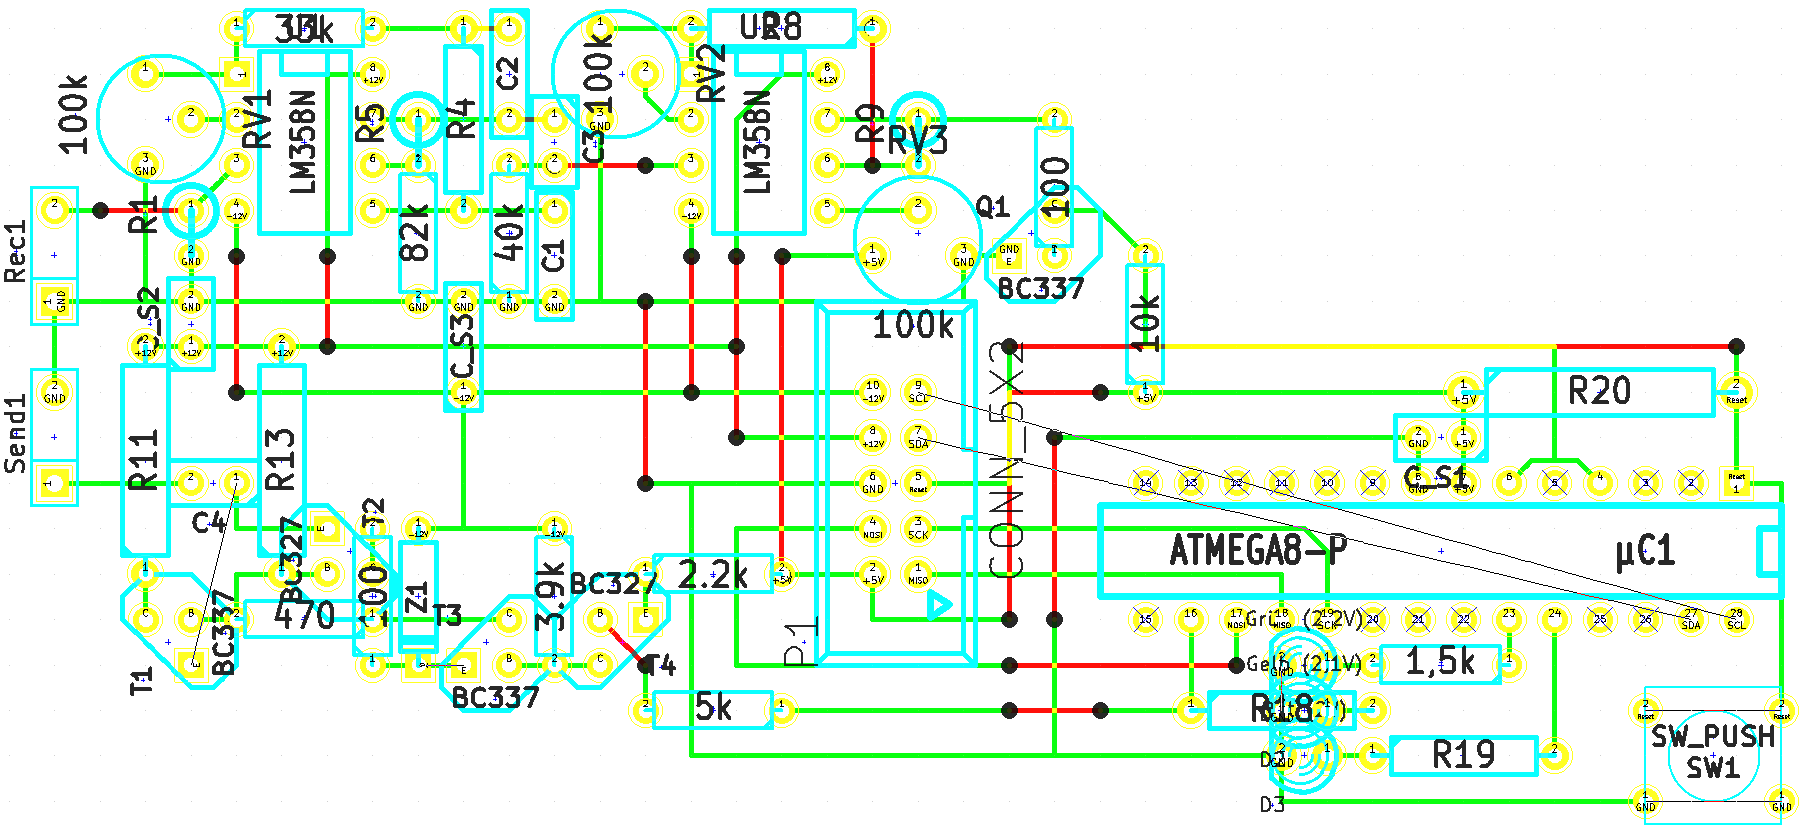
\includegraphics[width=(\textwidth)]{images/prototyp_2d.png}
	\caption{Prototyp-Platine mit Anzeige aus vier Ziffern} \label{img:prototype}
\end{figure}

\subsection{Aufbau}
Die Platine enthält die Sende- und Empfängerschaltung, den Mikrocontroller mit Anzeige-LEDs und Reset-Knopf, sowie eine Pfostenstecker-Buchse zur Verbindung mit der Verteilerplatine. Die Anzeige wurde nachträglich hinzugefügt. Obwohl der Platinenentwurf sehr Platzsparend ist, wurde versucht die Schaltungen räumlich voneinander zu trennen. Dadurch können Wechselwirkungen verhindert werden.\\
Als Sendeschaltung ist die Gegentaktstufe (siehe \ref{schaltung:gegentakt}) zum Einsatz gekommen, da sie die leistungsfähigste Sendeschaltung ist und die höchste Reichweite verspricht. Die Empfangsschaltung wurde mit der Pulsverstärkung und Frequenzfilterung realisiert (\ref{schaltung:pulse}), da die Nachteile zu diesem Zeitpunkt noch nicht bekannt waren. Zudem sollte die Platine als Vorführobjekt auch Geschwindigkeiten über den Dopplereffekt messen können, dafür müssen die Pulse einzeln detektierbar sein.

\begin{figure}[H]
	\centering
	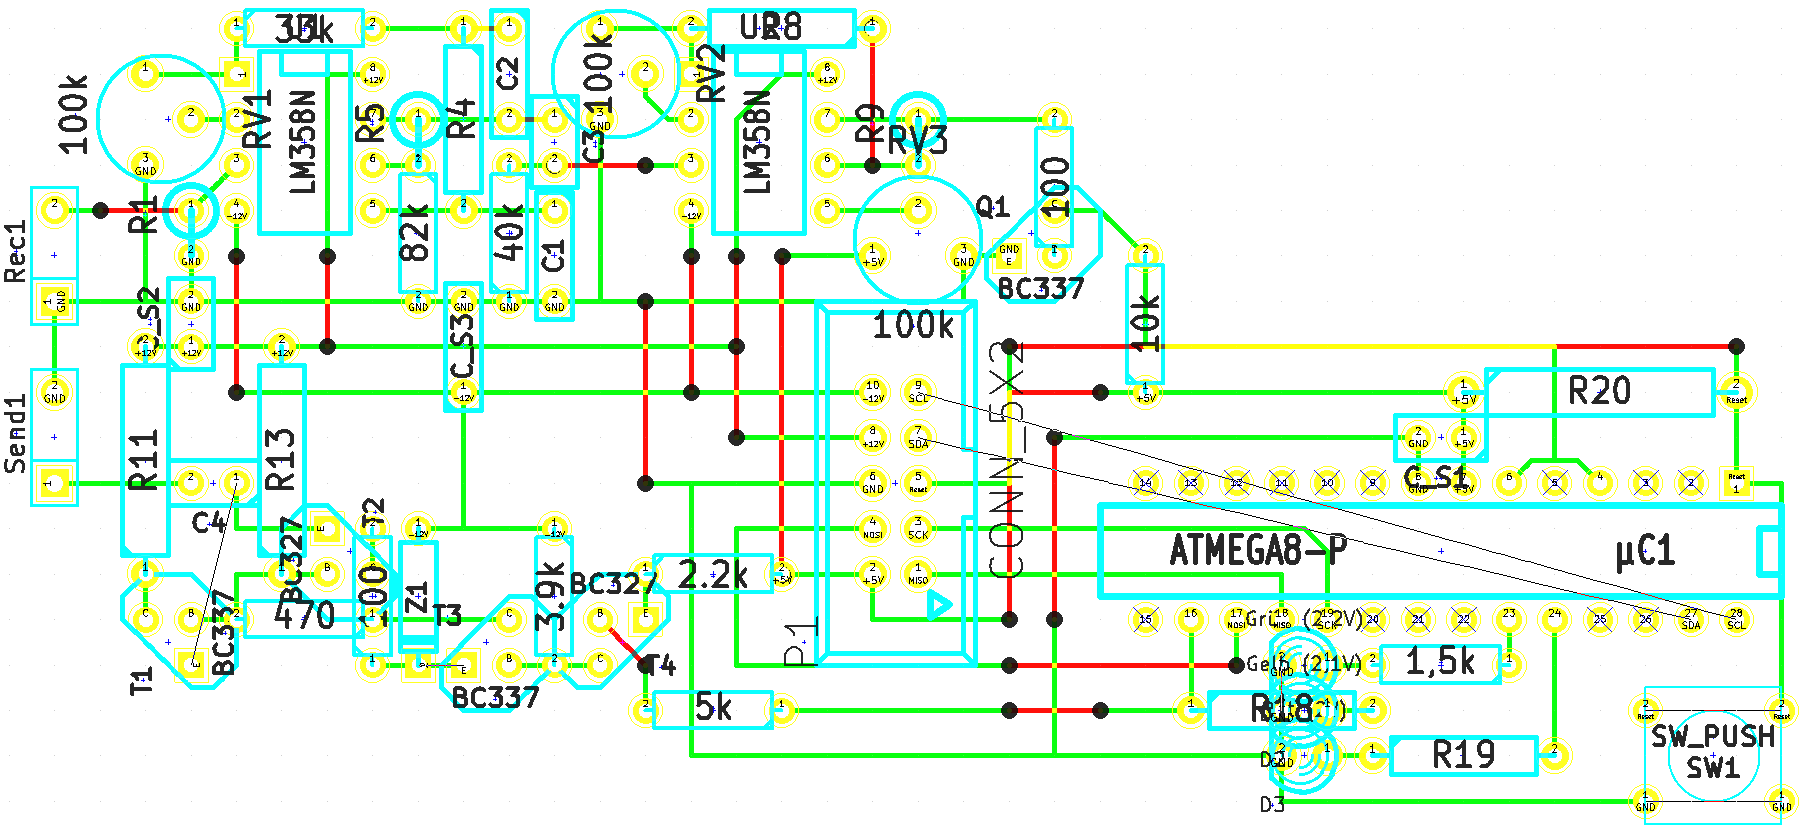
\includegraphics[width=(\textwidth)]{images/prototyp_2d.png}
	\caption{Platinenentwurf mit Sender, Empfänger und Mikrocontroller} \label{img:prototyp2d}
\end{figure}

\subsection{Probleme}
Das Löten des Platinenentwurfs stellte sich schwieriger heraus, als angenommen. Viele Komponenten wurden zu eng platziert, die Leiterbahnen waren zu verzweigt und es bestand die Gefahr eines Kurzschlusses. Außerdem wurden Sender und Empfänger zu nah aneinander platziert. Die Folge war, dass mechanische Schwingungen durch die Luft, aber auch über die Platine übertragen wurden. Abhilfe schaffte ein Stück Papier oder eine dünne Hartschaumplatte, die einen Großteil der Schwingungen reflektieren oder absorbieren lassen. Eine Totzeit zwischen Senden und Empfangen ließ sich dennoch nicht vermeiden, sodass die minimal messbare Distanz bei ca. $15cm$ liegt. Auch elektrische Wechselwirkungen wurden festgestellt. Zusätzliche Abblock-Kondensatoren direkt an der Stromversorgung der \acp{IC} konnten die Effekte eindämmen.


\section{Sensorplatinen}
Die Sensorplatinen sind verkleinerte Versionen der Prototyp-Platine, wobei die Schaltungen durch die gesammelten Erkenntnisse verbessert und vereinfacht wurden. Anders als die Prototyp-Platine sind sie nicht mit einer Anzeige ausgestattet, sodass ein Betrieb ohne Kommunikationsverbindung per \ac{TWI} nicht möglich ist. Es gibt zwei Sensorplatinen, die zusammen mit der Prototyp-Platine für die Positionsbestimmung eingesetzt werden. Die Pinbelegung des Verbindungssteckers ist identisch mit der vorherigen Platine.

\begin{figure}[H]
	\centering
	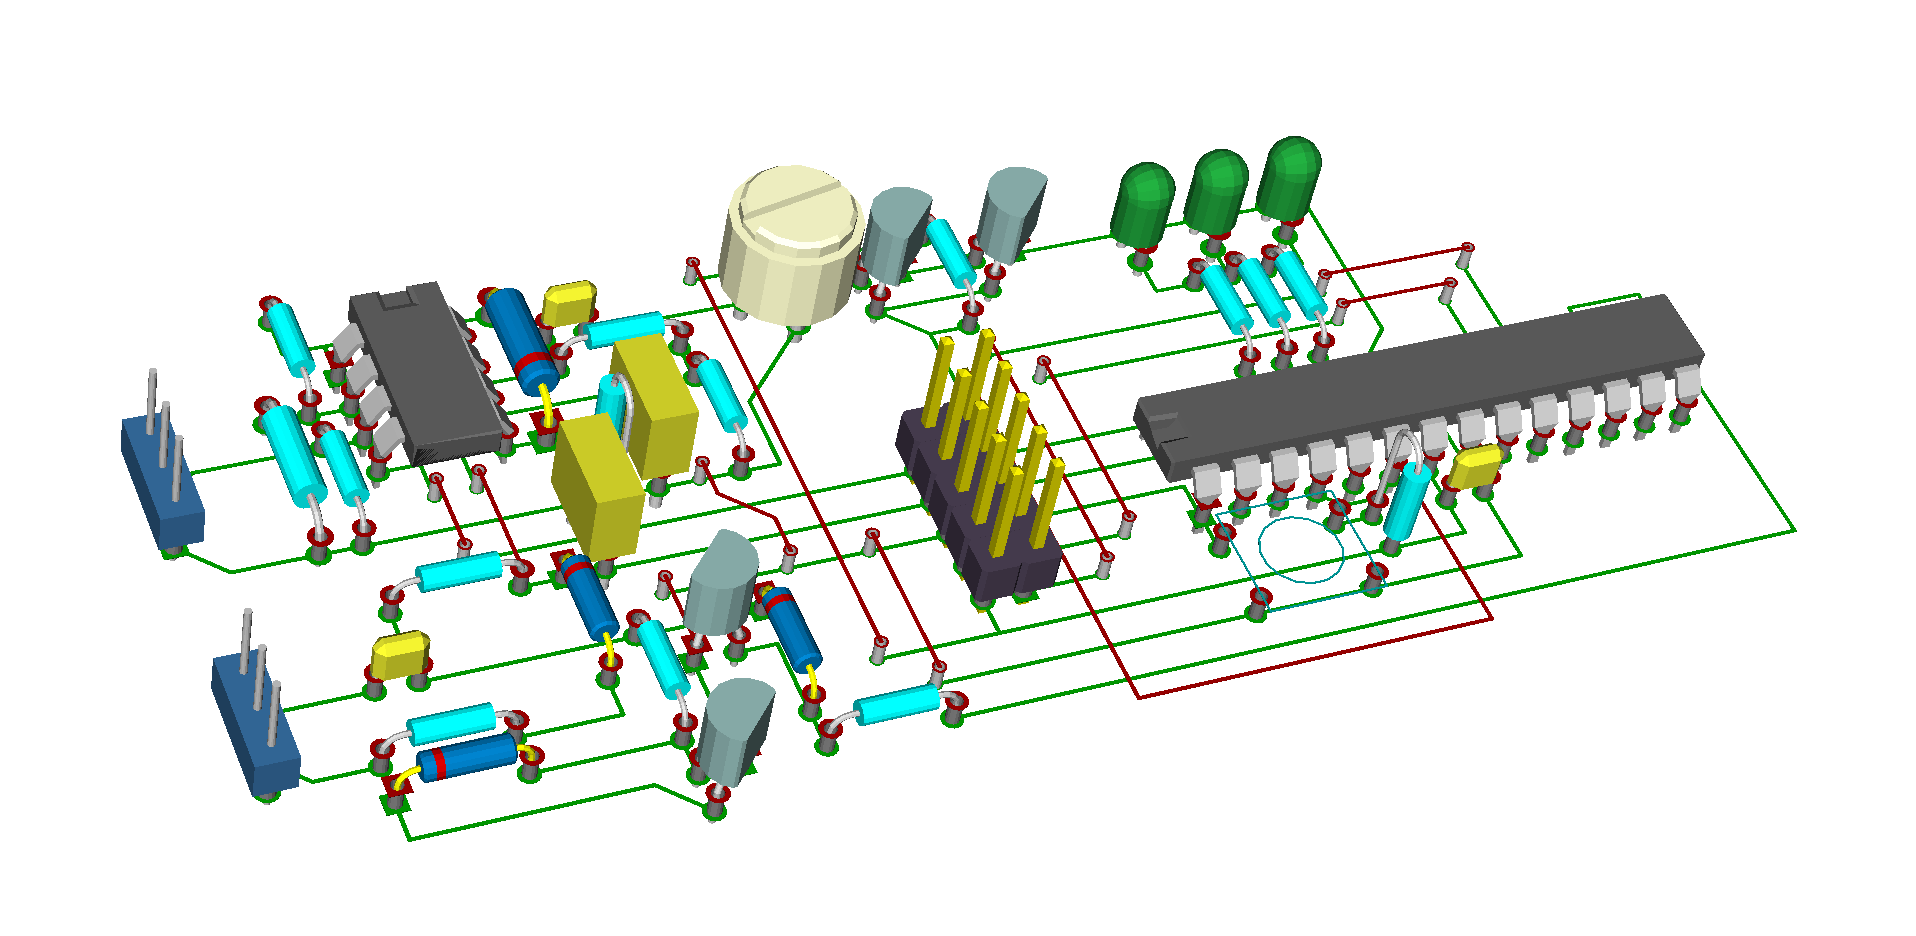
\includegraphics[width=(\textwidth)]{images/endplatine_3d.png}
	\caption{Platinenentwurf als 3D-Darstellung} \label{img:endplatine3d}
\end{figure}


\subsection{Änderungen der Schaltungen}



\section{Verteiler-Platine und Verkabelung}



%TODO Fehler mit Triggersignal
	%!TEX root = ../dokumentation.tex

% Kapitel über Firmware des Mikrocontrollers
% Sprache, Funktionen, Schnittstellen, ...


\chapter{Firmware}
Als Firmware wird die Software bezeichnet, welche auf dem Mikrocontroller ausgeführt wird. Sie läuft ohne Betriebssystem direkt auf der Hardware und kann in Assembler, C oder anderen hardwarenahen Programmiersprachen geschrieben werden. In diesem Fall wurde sie mit C und den dazugehörigen Bibliotheken für die AVR-Mikrocontroller entwickelt.\\
Die Firmware hat die Aufgabe die Hardware des Controllers zu steuern. Sie ist in Module aufgeteilt, die jeweils für eine Hardwarekomponente zuständig sind:
\begin{description} %TODO Eigene Überschriften statt description?
	\item[LED-Statusanzeige:] \hfill \\Die LEDs werden über die \ac{GPIO}-Pins des AVR angesteuert. Per Software-\ac{PWM} lassen sich auch sanft pulsierende Signale realisieren. Damit kann der Controller mitteilen, in welchem Zustand er sich befindet und dass die Firmware nicht hängen geblieben ist.
	\item[7-Segment-Anzeige:] Die Platine mit den vier 7-Segment-Ziffern zur Anzeige von Messergebnissen benötigt ein extra Modul, um diese Anzusteuern. Das geschieht über eine serielle Verbindung zu vier hintereinander geschalteten Schieberegistern. Die Werte werden per \ac{Bitbanging} über die \ac{GPIO}-Pins in die Register geschoben, diese haben parallele Ausgänge, die mit den Ziffern verbunden sind.
	\item[Signalerzeugung mit \ac{PWM}:] Das $40kHz$-Signal für den Ultraschallsender wird von der Mikrocontroller-Hardware erzeugt. Dazu wird ein Zähler benötigt, der bei einem Vergleichswert und beim Überlauf den Pegel eines Ausgangspins setzt. Die Firmware initialisiert und startet den Timer, die Erzeugung des Signals wird ausschließlich von der Hardware erledigt. Dadurch wird das Signal sehr präzise und die Rechenleistung des Mikrocontrollers steht für andere Zwecke zur Verfügung.
	\item[Laufzeitmessung:] Für eine präzise Zeitmessung wird ein weiterer Hardwarezähler verwendet. Er wird in einer konstanten Frequenz inkrementiert, bis das Signal eingetroffen ist. Wenn das Zählerregister zu klein ist, kann bei einem Überlauf ein weiteres Register inkrementiert werden, damit die Messgenauigkeit und -Reichweite nicht durch die Software eingeschränkt werden müssen.
	\item[Signalerkennung:] Empfängt der Ultraschallempfänger ein Signal, so erhält der Mikrocontroller einen digitalen Puls. Auf einem Interrupt-Eingang löst die Flanke dieses Signals einen Sprung in der Firmware aus, sodass der Hardwarezähler sofort gestoppt werden kann. Ein Interrupt erhöht die Präzision der Messungen, da die Software alleine nur sequentiell den Signalpegel abfragen könnte und die Zeitpunkte ungenau werden. Zudem können die Flanken nicht aufgrund anderer Rechenaufwänden verpasst werden.
	\item[\ac{TWI}-Kommunikation:] Die serielle Schnittstelle wird verwendet, um mit dem Raspberry Pi zu kommunizieren. Als Slave muss der Controller auf Anfragen reagieren, es können Messungen angefordert und Ergebnisse ausgelesen werden. Die AVR-Mikrontroller besitzen eine \ac{TWI}-Hardware, die von der Firmware genutzt wird.
\end{description}


\section{Genauigkeit und Reichweite der Messungen}
Die Messgenauigkeit und maximale Reichweite ist durch den Takt des Zählers, sowie die Bitbreite des Messwertes abhängig. Die Firmware taktet den Zähler mit $1MHz$ und speichert die Daten in einem 16-Bit Register. Daraus ergeben sich folgende Werte:\\
Schrittlänge:
\begin{equation} %TODO Schallgeschwindigkeit zw 20-25° 344-245 m/s, Außerdem: Pro gemessene Strecke wird doppelte Schallstrecke benötigt
\Delta s = \frac{u}{f} = \frac{0.5 * 343m/s}{1*10^6 1/s} = 0.172 mm
\end{equation}
Maximale Distanz:
\begin{equation}
dist = 2^{16} * \Delta s = 11.24 m
\end{equation}

Der Wert bezieht sich auf die relative Genauigkeit. Offsetfehler, die durch Latenzzeiten entstehen, können in einem gewissen Umfang experimentell bestimmt und herausgerechnet werden. Die relative Genauigkeit hängt allerdings von der Toleranz des internen Taktes ab, dieser wird vor allem bei Temperaturänderungen ungenauer. Bei starken Abweichungen kann der Mikrocontroller über einen genaueren externen Quarz getaktet werden.

\section{Erkennung der Platine durch die Firmware}


\section{Laufzeitmessung zwischen den Platinen}


%TODO: Ablaufdiagramm
	%!TEX root = ../dokumentation.tex

\chapter{Schnittstellenkommunikation}
In eingebetteten Systemen sind Sensoren und Aktoren erfolgt deren Anbindung oft mittels eines I\textsuperscript{2}C-Busses. Dies unterstützt Linux auf dem Raspberry Pi mit einem eigenen Subsystem. I\textsuperscript{2}C ist ein serieller Master-Slave-Datenbus, der über eine Datenleitung (SDA) und eine Taktleitung (SCL) verfügt und mit einer 7-Bit-Adresse 112 Geräte (Slaves) ansprechen kann. Für den Datenaustausch zwischen dem Raspberry Pi und dem ATMega8-Mikrocontroller kann man das I\textsuperscript{2}C/TWI-Übertragungsprotokoll nutzen.TWI steht für Two-Wire-Interface (TWI) und überträgt Daten seriell.
Beim Verbinden des AVR mit dem RPi muss darauf geachtet werden, dass der AVR mit 3,3V läuft, da ansonsten der Raspberry Pi beschädigt wird.\\
Im Anschluss daran muss der Raspberry Pi zur Kommunikation per I\textsuperscript{2}C als Master (Module hinzufügen und Installation des I\textsuperscript{2}C-Tools-Pakets) und der ATmega als I\textsuperscript{2}C-Slave vorbereitet werden. Außerdem muss die nötige I\textsuperscript{2}C-Bibliothek eingebunden werden.\\
Um die Verbindung herzustellen wird SDA und SCL des Raspberry (Pin 3 und 5) jeweils mit SDA und SCL des AVR verbunden. Dies entspricht beim ATmega8 Pin 27 und 28. Im nächsten Schritt werden die Leitungen über einen Pull-up-Widerstand mit Vcc verbunden.
Es muss dabei beachtet werden, dass der im Raspberry Pi verwendete Broadcomm BCM2835 Prozessor einen Fehler auslösen kann, der dazu führt, dass eine Kommunikation mit einigen I\textsuperscript{2}C Geräten unmöglich wird. In diesem Fall werden falsche Daten gelesen oder geschrieben. Der Grund hierfür ist, dass einige I\textsuperscript{2}C Geräte „clock stretching“ verwenden, welches nicht durch den Raspberry unterstützt wird. 

\section{Detaillierte Problembeschreibung} \label{clockstretching}
Clock Stretching: Gemäß ihrer Spezifikation können I\textsuperscript{2}C-Slaves während einer Kommunikation die Clock-Leitung auf "low" halten. Auf Weise wird ein erneutes Steigen der Flanke verhindert und die Übertragung kann aktiv verzögert werden. Falls nötig ist so mehr Zeit für die Verarbeitung der Daten vorhanden. Gibt der I\textsuperscript{2}C die Clock Leitung dann wieder frei, ist es notwendig, dass der Master den Takt wieder an die Clock-Leitung anlegt.

Der eigentliche Fehler besteht also darin, dass die SCL Taktleitung nur maskiert wird sobald ein I\textsuperscript{2}C Slave die Taktleitung auf „low“ zieht. In der Folge stellt der Raspberry Pi allerdings nicht sicher, dass der folgende Takt die gleiche Länge besitzt. Es entstehen Spikes, die dann die Kommunikation mit dem I\textsuperscript{2}C Gerät unmöglich machen, da diese zu kurz sein können um vom I\textsuperscript{2}C-Slave erkannt zu werden. Das kann zu einer Verschiebung des Taktzyklus führen, sodass Master und Slave nicht mehr synchron laufen. \\
Dadurch entsteht ein weiteres Problem: der Raspberry liest die Datenleitung zu früh ein (noch während der Slave die Leitung auf „low“ hält) und selbst sehr kurze Clock-Stretching führen dazu, dass falsche Daten vom Raspberry gelesen werden.

Es gibt mehrere Möglichkeiten dieses Problem zu umgehen:
\begin{itemize}
	\item keine I\textsuperscript{2}C Geräte nutzen, die Clock-Stretching einsetzen
	\item clock-stretching nur am Ende nach dem Lesen des ACK/NACK verwenden, und ihn dabei um mindestens 1/2 Takt-Periode verlängern
	\item einen geringeren I\textsuperscript{2}C-Takt wählen, so dass die I\textsuperscript{2}C-Slaves schnell genug sind, und kein Clock-Stretching mehr benötigen
\end{itemize}
Im Rahmen dieser Arbeit wurde daher zunächst beschlossen, Clock-Stretching durch den I\textsuperscript{2}C-Slave zu unterbinden, da diese ohnehin nicht benötigt werden. Möglich wird dies durch Anpassungen in der Firmware (diese arbeitet nun mit Interrupts und daher viel schneller) und eine verringerte Frequenz am Raspberry.


\begin{figure}[H]
	\centering
	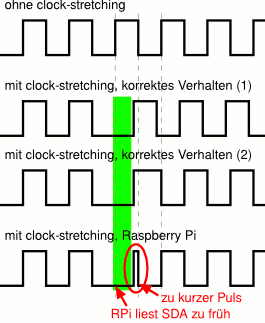
\includegraphics[scale=0.8]{images/rpi-i2c-bug.png}
	\caption{Clock-Stretching beim Raspberry Pi\footnotemark}
\end{figure}
\footnotetext{\url{http://www.advamation.de/technik/raspberrypi/rpi-i2c-bug.html}}

\section{Genutztes Protokoll}
Das erstellte Protokoll legt das Format, den Inhalt, die Bedeutung und die Reihenfolge gesendeter Nachrichten fest. Dies regelt den Ablauf und gleichzeitig wird eine Dokumentation darüber sichergestellt:
Es wird immer ein Byte gesendet. Dieses Byte repräsentiert einen Befehl:
Einzelheiten der vorhandenen Befehle 
(Gliederung: <Name> <Hex> <Beschreibung>)):
\begin{enumerate}
	\item PROT\_CONNECT 0x01: Verursacht einen Statuswechsel: Der Controller wartet auf die Messbefehle. Zusätzlich ist es mit Hilfe dieses Befehls möglich den Zustand des Controllers zurücksetzen.
	\item PROT\_DISCONNECT 0x02: Erneuter Statuswechsel: Controller kann nun selbstständig Messen und erwartet keine Befehle.
	\item PROT\_STARTMES 0x11: Befehl eine Laufzeitmessung zu starten, Ergebnis wird vom Mikrocontroller gepuffert.
	\item PROT\_DIST\_SEND 0x21: Sendet gleichzeitig ein Trigger-Signal und einen Ultraschallimpuls -> Wird von einem Controller ausgeführt um die Distanzen untereinander auszuessen.
	\item PROT\_DIST\_MES 0x22: Versetzt den Mikrocontroller in einen Wartezustand. Die Laufzeitmessung beginnt mit dem empfangenen Trigger-Signal. Das Ergebnis wird gepuffert. Das Kommando muss bei den beiden Controllern ausgeführt werden, bevor die dritte Platine das Kommando PROT\_DIST\_SEND erhält.
\end{enumerate}
Der Master (RPi) kann zu jedem Zeitpunkt Daten anfordern. Gesendet werden kann Folgendes:
\begin{enumerate}
	\item PROT\_MESSUCC 0x15: Wenn die Messung erfolgreich war, folgen 2 Byte (uint16) Messdaten in der Einheit mm. 
	\item PROT\_MESFAIL 0x16: Wenn die Messung fehlgeschlagen ist (kein Signal empfangen), folgen keine weiteren Daten.
	\item PROT\_NODATA 0x51: Dabei handelt es sich um einen Fehlercode: Der Controller verfügt über keinerlei Messdaten. Entweder wurde keine Messung gestartet, oder sie wurde noch nicht beendet.
\end{enumerate}
Die maximale Dauer einer Messung beträgt $66 ms$ ($2^{16} Bit / 1000000 Hz, 344m/s * 66ms = ca. 22m$). Diese Zeitspanne muss abgewartet werden, bis die Daten angefordert werden können und eine weitere Messung (anderer oder selber Controller) gestartet werden kann. Die drei Controller haben für den I\textsuperscript{2}C-Bus folgende Adressen abhängig von den Platinen fest zugeordnet: 0x2a, 0x2c, 0x2e.


	%!TEX root = ../dokumentation.tex

% Inhalt 1:1 von Christian Buss übernommen

\chapter{Oberflächenprogrammierung}
Eine weitere Anforderung der Studienarbeit stellt die Visualisierung des gemessenen Gegenstandes dar. Dies wurde in Form eines Dialoges umgesetzt. Dazu wurden im Vorfeld Recherchen durchgeführt um die beste Komptabilität vom Dialog mit dem Raspberry Pi zu sicherzustellen. Mit Qt programmierte Dialoge habe ein gute Kommunikation mit dem Raspberry Pi. Infolgedessen wurde auf einer virtuellen Maschine ein Linux-Betriebssystem installiert, da auf dem Raspberry Pi Linuxbasierte Betriebssysteme sehr gut laufen. Auf diesem Betriebssystem wurde die Entwicklungssoftware Qt-Creater installiert. Die Software benutzt die Qt-Bibliothek, eine C++-Klassenbibliothek für die Programmierung von grafischen Benutzeroberflächen. 
Für den Dialog wurde zuerst ein einfacher Dialog angelegt. Auf diesem wird mithilfe von Zeichen-Events ein Raster gezeichnet das später zu Orientierung dienen soll. Zusätzlich werden drei Buttons eingefügt:
\begin{itemize}
	\item einer zum Schließen des Fensters
	\item einer zum Lokalisieren der Sensoren
	\item einer zum Starten der Messung.
\end{itemize}
Beim Klick auf den Lokalisierungs-Button wird ein Signal an die Sensoren gesendet welche dann den Abstand zueinander zurückgeben. Auf dieser Grundlage werden die jeweiligen Positionen ermittelt Dabei werden zwei der Sensoren auf bestimmte Koordinaten festgesetzt um die dritte Sensorposition besser bestimmen zu können. Die Abstände zwischen den Sensoren bilden die Seiten des Dreieck (Siehe \ref{img:gui1}), dadurch kann dann der Winkel Alpha berechnet werden. Mit diesem Winkel und der Seite b kann die Höhe h berechnet werden. Jetzt kann der Satz des Phytagoras angewendet werden um $c_2$ zu berechnen. Dann muss nur noch h auf die y-Koordinaten und $c_2$ auf die x-Koordinaten addiert werden.
\begin{figure}
	\centering
	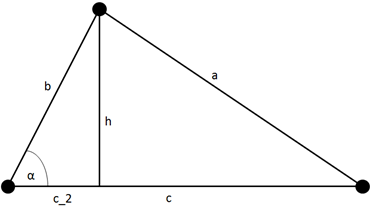
\includegraphics[scale=1]{images/gui/01.png}
	\caption{Berechnung der Sensorenpostion} \label{img:gui1}
\end{figure}

Sobald die Abstände bekannt sind werden die Positionen in dem Raster angezeigt. Da das Raster aus 16 Kasten besteht muss ein bestimmter Maßstab angegeben, dieser wird mittels der Abstände der Sensoren zueinander berechnet und neben einem Kasten zusätzlich dargestellt.\\
Mit betätigen des Buttons zum Starten der Messung wird ein Befehl an die Sensoren gesendet, diese geben dann einen Abstand zum Gegenstand zurück. Mit diesen Abständen wird eine Berechnung durchgeführt um die korrekte Position des Gegenstandes zu ermitteln. Die Abstände zum Gegenstand teilen das Dreieck nochmals in drei kleinere Dreiecke auf. Im nächsten Schritt werden die Winkel zum Ursprung berechnet, dadurch lässt sich die Steigung berechnen. Die Steigung sowie ein Punkt eines Sensors wird in die Geradengleichung eingesetzt und es kann der Startpunkt auf der Y-Achse berechnet werden. Somit kann die Geradengleichung aufgestellt werden. Dies wird für jeden Abstand durchgeführt, damit können durch das Gleichsetzten zweier Geradengleichungen der Schnittpunkt dieser ermittelt werden. Durch zweimaliges Wiederholen werden drei Schnittpunkte ermittelt, diese werden verglichen wenn die Abweichungen vernachlässigbar klein sind wird der Gegenstand im Raster angezeigt.
\begin{figure}[H]
	\centering
	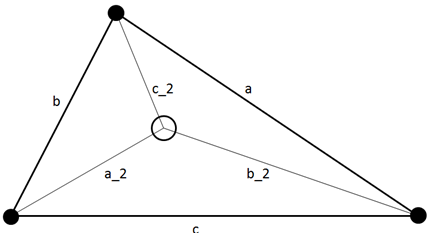
\includegraphics[scale=1]{images/gui/02.png}
	\caption{Berechnung der Position des Gegenstandes} \label{img:gui2}
\end{figure}

Wenn die Berechnung durchgeführt worden ist wird ein Kreis in das Raster gezeichnet um den Gegenstand zu symbolisieren. In Abbildung 3 zu sehen ist der Dialog.\\
Dieser Dialog wird dann auf dem Raspberry Pi gestartet und von diesem aus bedient und benutzt. Zu diesem Zweck wurde auf dem Raspberry Pi das Betriebssystem Rasbian installiert da dieses sehr einfach zu bedienen ist. Sobald der Raspberry Pi gestartet und an einen Bildschirm angeschlossen ist kann der Dialog einfach gestartet werden.

\begin{landscape}
	\begin{figure}
		\centering
		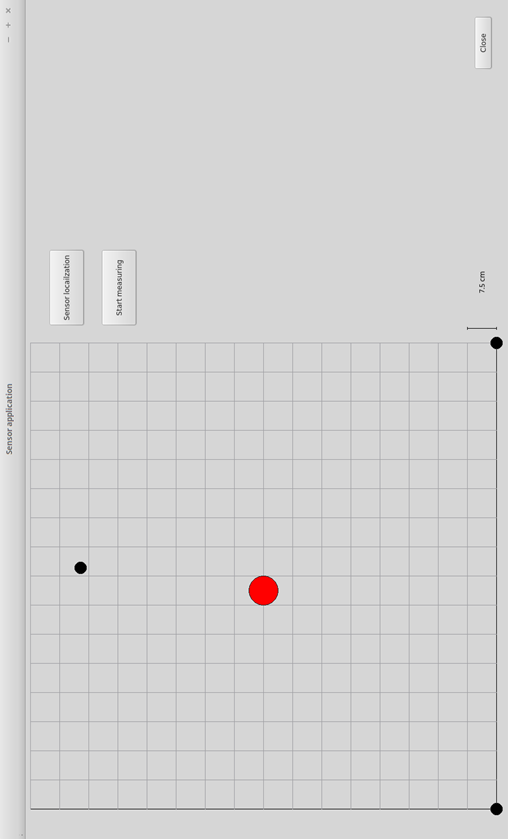
\includegraphics[width=(0.9\textwidth), angle=270]{images/gui/03.png}
		\caption{Dialog zur Darstellung der Sensoren und des Gegenstandes} \label{img:gui3}
	\end{figure}
\end{landscape}

	%!TEX root = ../dokumentation.tex

\chapter{Funktionstest}

 % Messergebnisse, Genauigkeit, Zuverlässigkeit
	%!TEX root = ../dokumentation.tex

\chapter{Inbetriebnahme}

%TODO Bild von kompletten Aufbau
Der Bildschirm muss an den HDMI-Ausgang des Raspberry Pi angeschlossen werden (weißes Kabel). Anschließend wird das Flachbandkabel der Verteiler-Platine befestigt. Die Seite mit der roten Leitung muss bündig auf die Pins gesteckt werden, auf der anderen Seite bleiben einige Pins unbenutzt. Anschließend kann die Stromversorgung über das Mikro-USB-Kabel hergestellt werden (schwarzes Kabel). Der Computer startet daraufhin automatisch.\\
\begin{figure}[H]
	\centering
	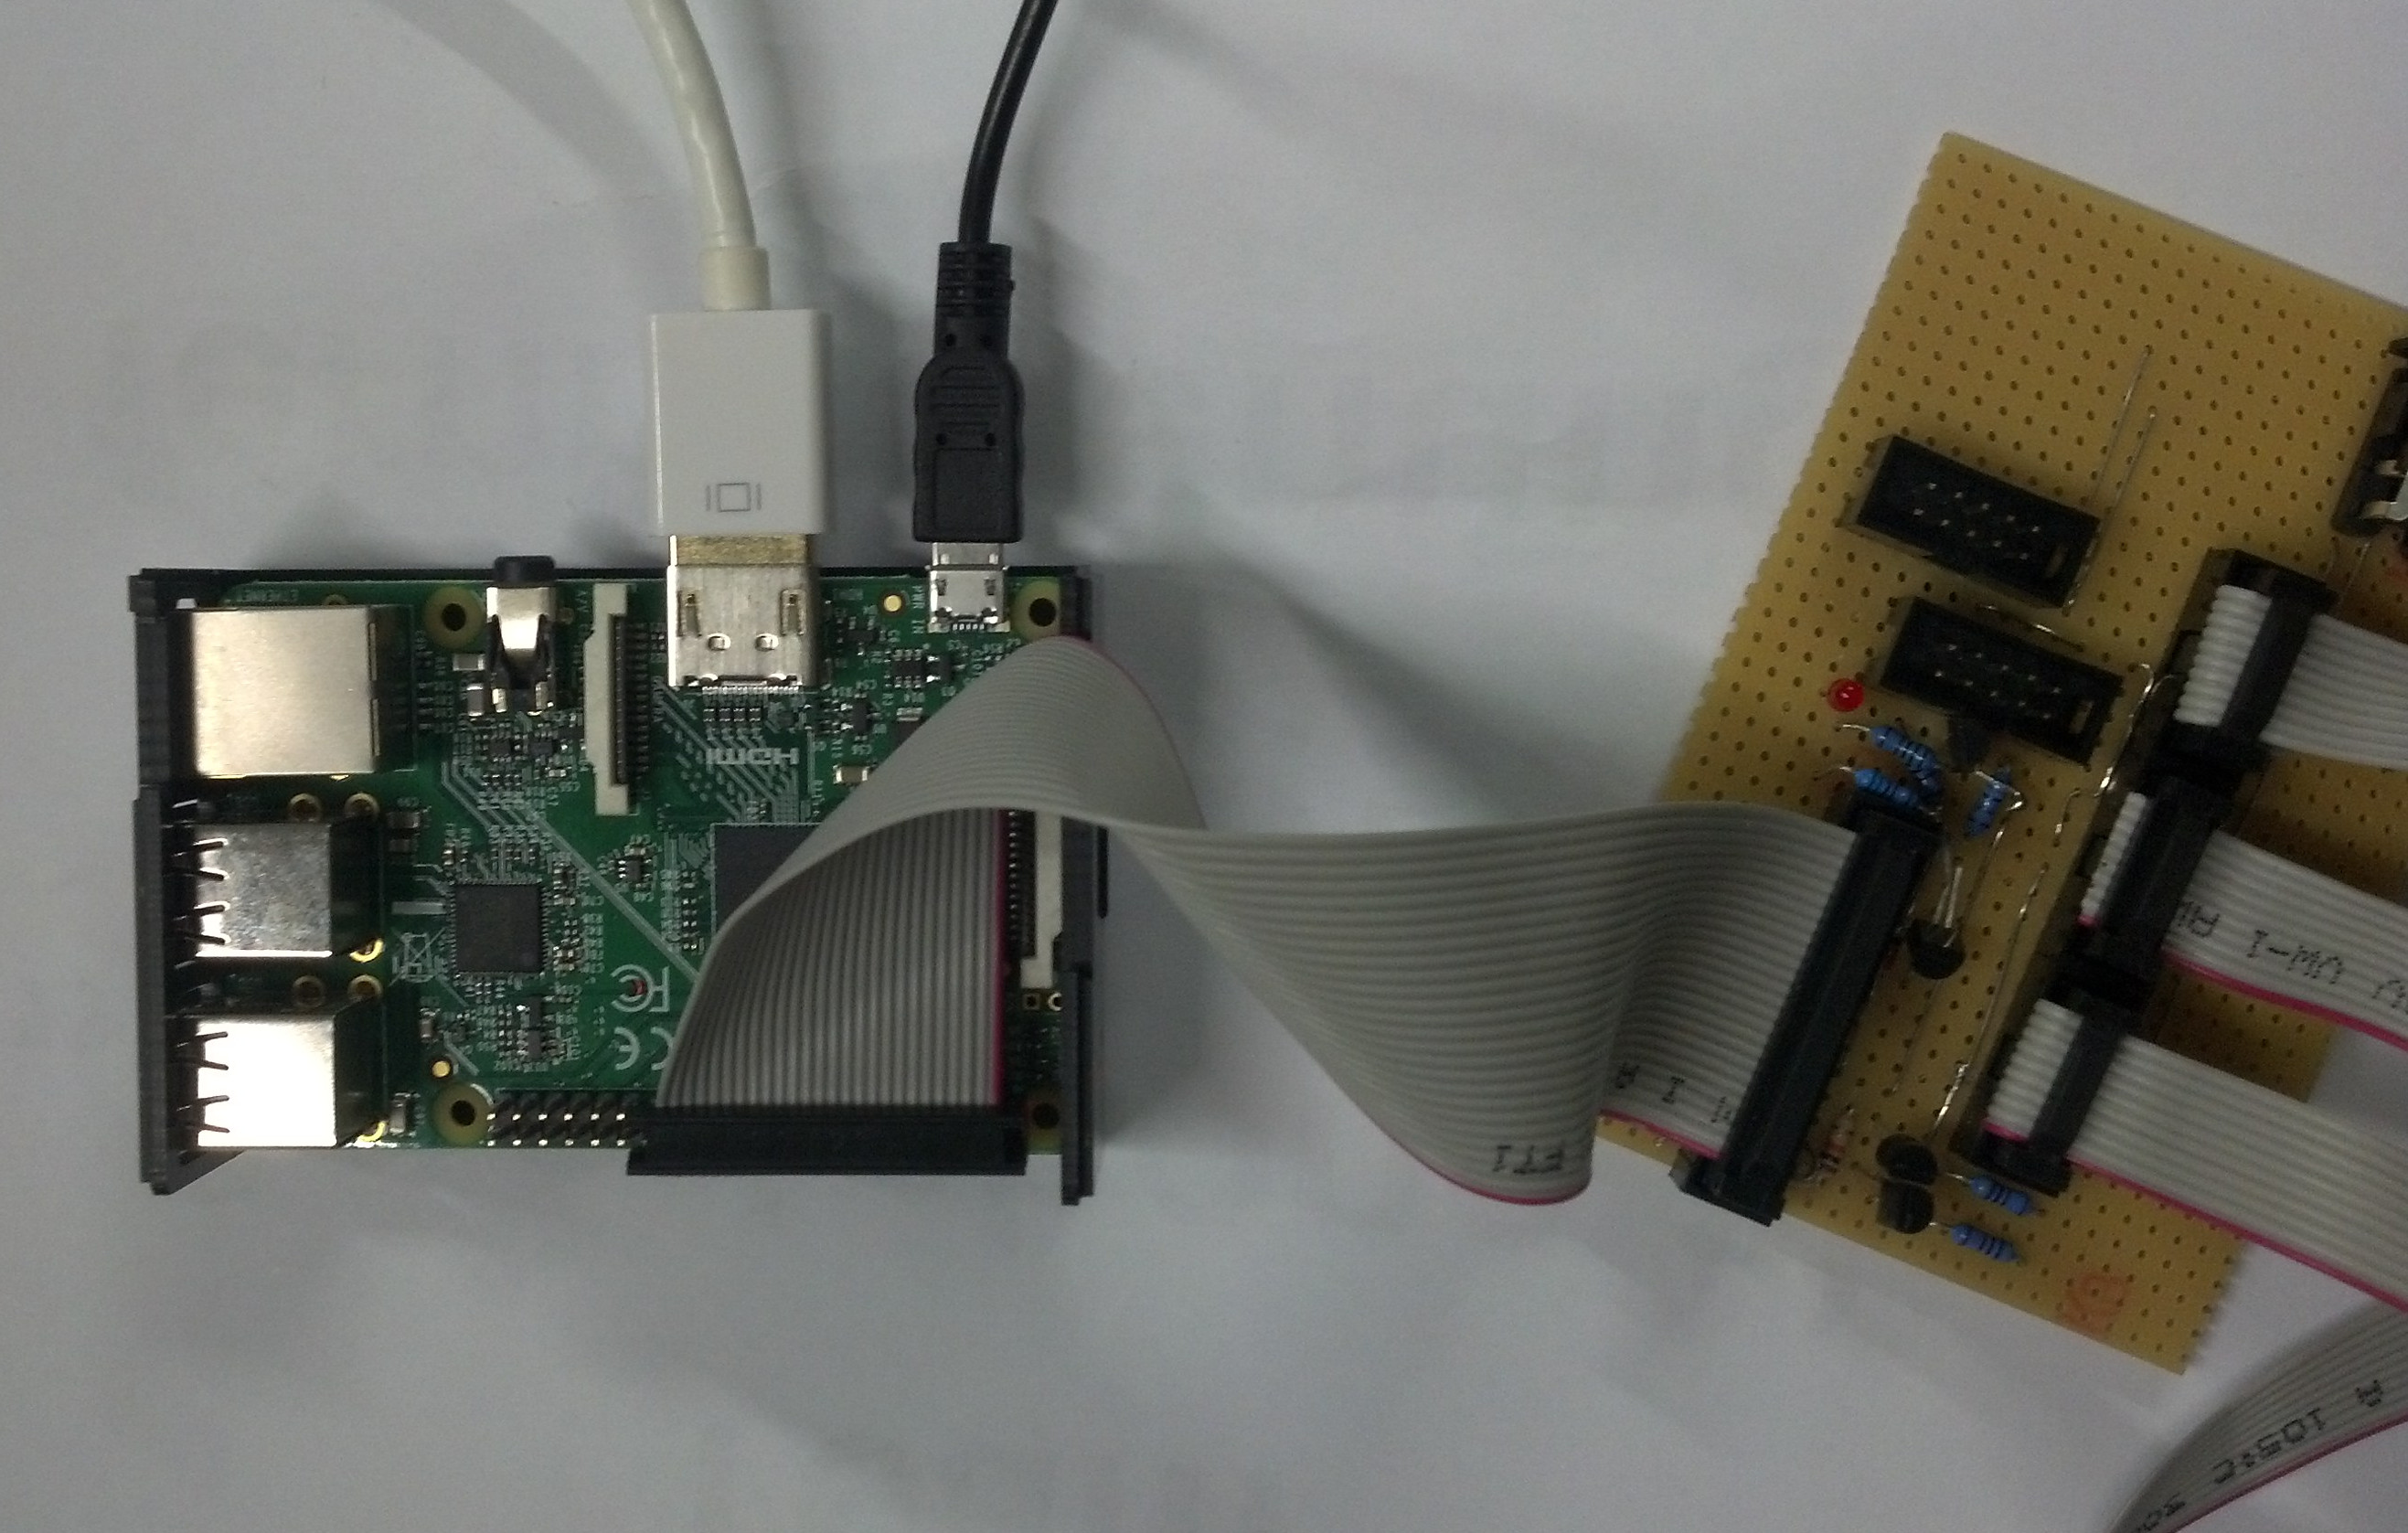
\includegraphics[width=(\textwidth), angle=0]{fotos/rasp.jpg}
	\caption{Verkabelung des Raspberry Pi} \label{p:1}
\end{figure}
Die drei Sensorplatinen werden auf den oberen drei kleinen Steckplätzen der Verteiler-Platine befestigt, die Reihenfolge spielt dabei keine Rolle. Die übrigen zwei Steckplätze wurden verwendet, um die Mikrocontroller zu programmieren und werden nicht mehr benötigt. Anschließend wird die Stromversorgung eingesteckt, woraufhin die Platinen einige Signale über die LEDs ausgeben. Die kleinen Sensorplatinen wechseln in den Wartezustand, bis eine Verbindung mit ihnen aufgebaut wird (rote LED pulsiert). Die große Sensorplatine führt automatisch Distanzmessungen aus und zeigt die Ergebnisse auf der 7-Segment-Anzeige an. Sobald eine Verbindung (z.B. über die GUI) aufgebaut wurde, stoppen die automatischen Messungen, damit es zu keinen Signalüberlagerungen während der Positionsbestimmung kommt. Die Mikrocontroller können über den Reset-Knopf in ihren Ausgangszustand zurück gebracht werden.\\
\begin{figure}[H]
	\centering
	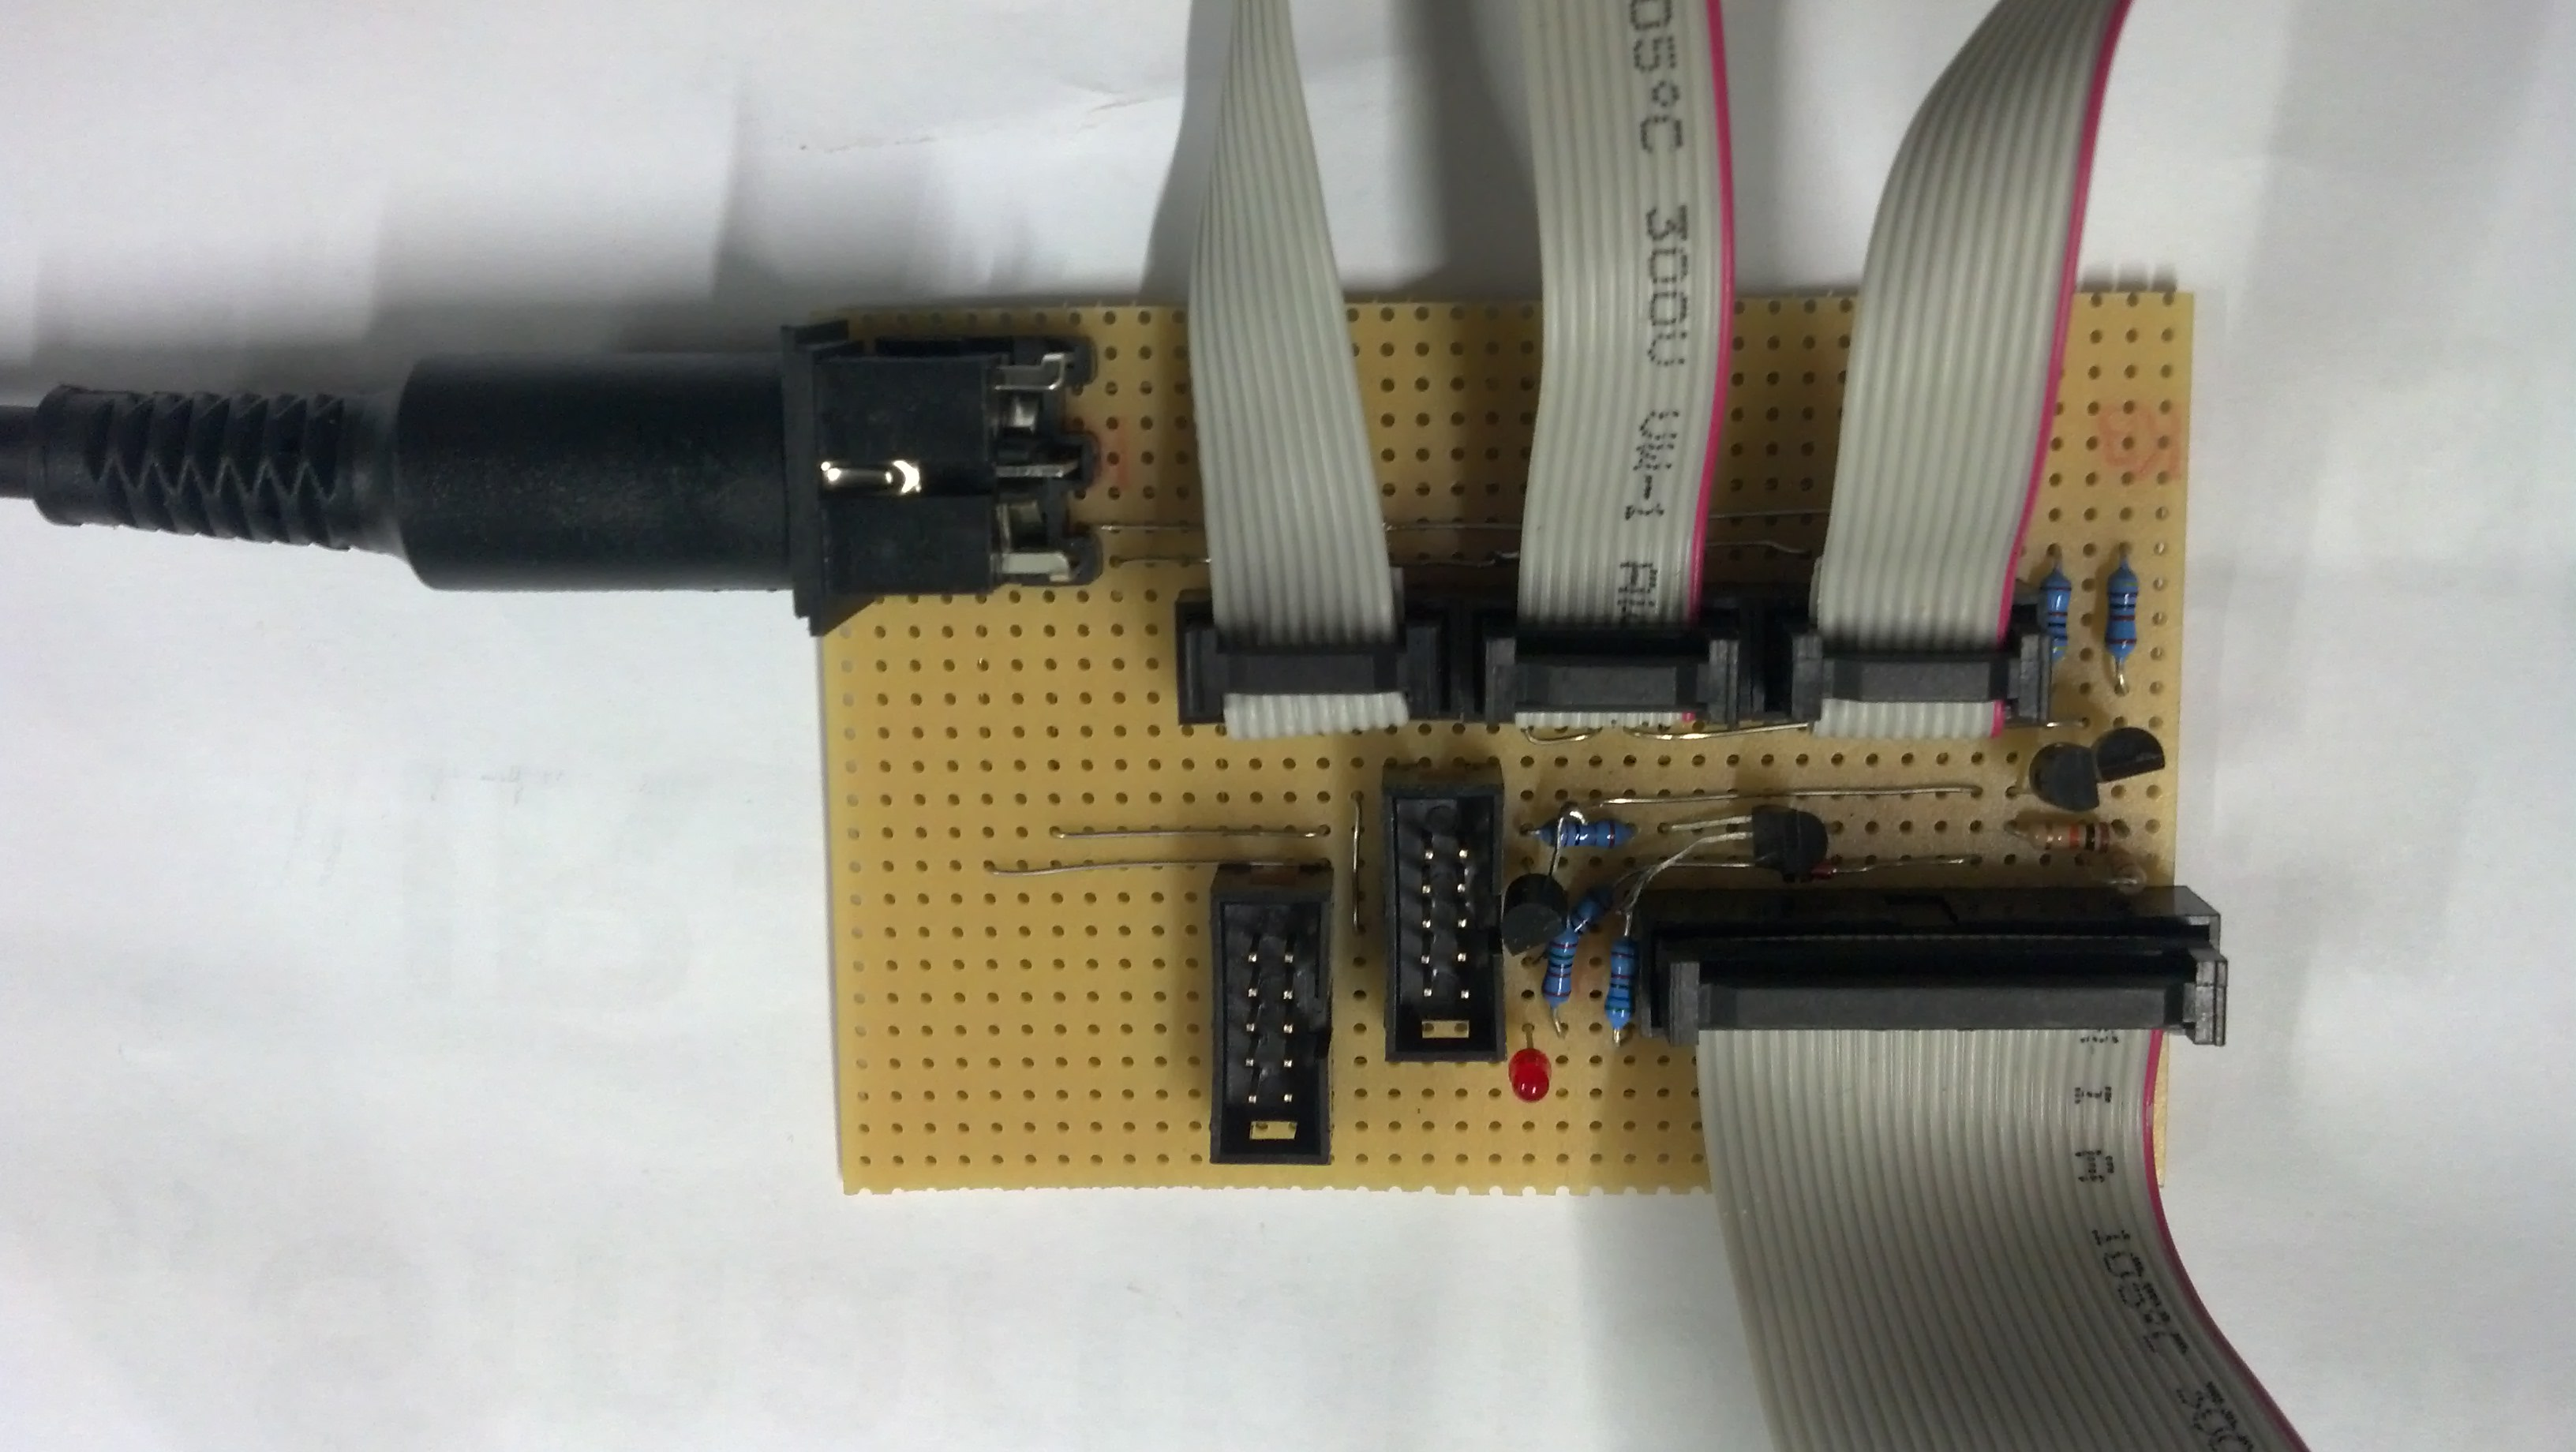
\includegraphics[width=(\textwidth), angle=0]{fotos/verteiler.jpg}
	\caption{Steckplätze der Verteiler-Platine} \label{p:2}
\end{figure}
Bei der Positionsbestimmung werden die Platinen in einem Dreieck angeordnet. Sie sind nummeriert und müssen gegen den Uhrzeigersinn geordnet sein. Positionen können innerhalb der eingespannten Fläche bestimmt werden, wobei eine Distanz von $15cm$ zu den Platinen eingehalten werden muss. \\
\begin{figure}[h]
	\centering
	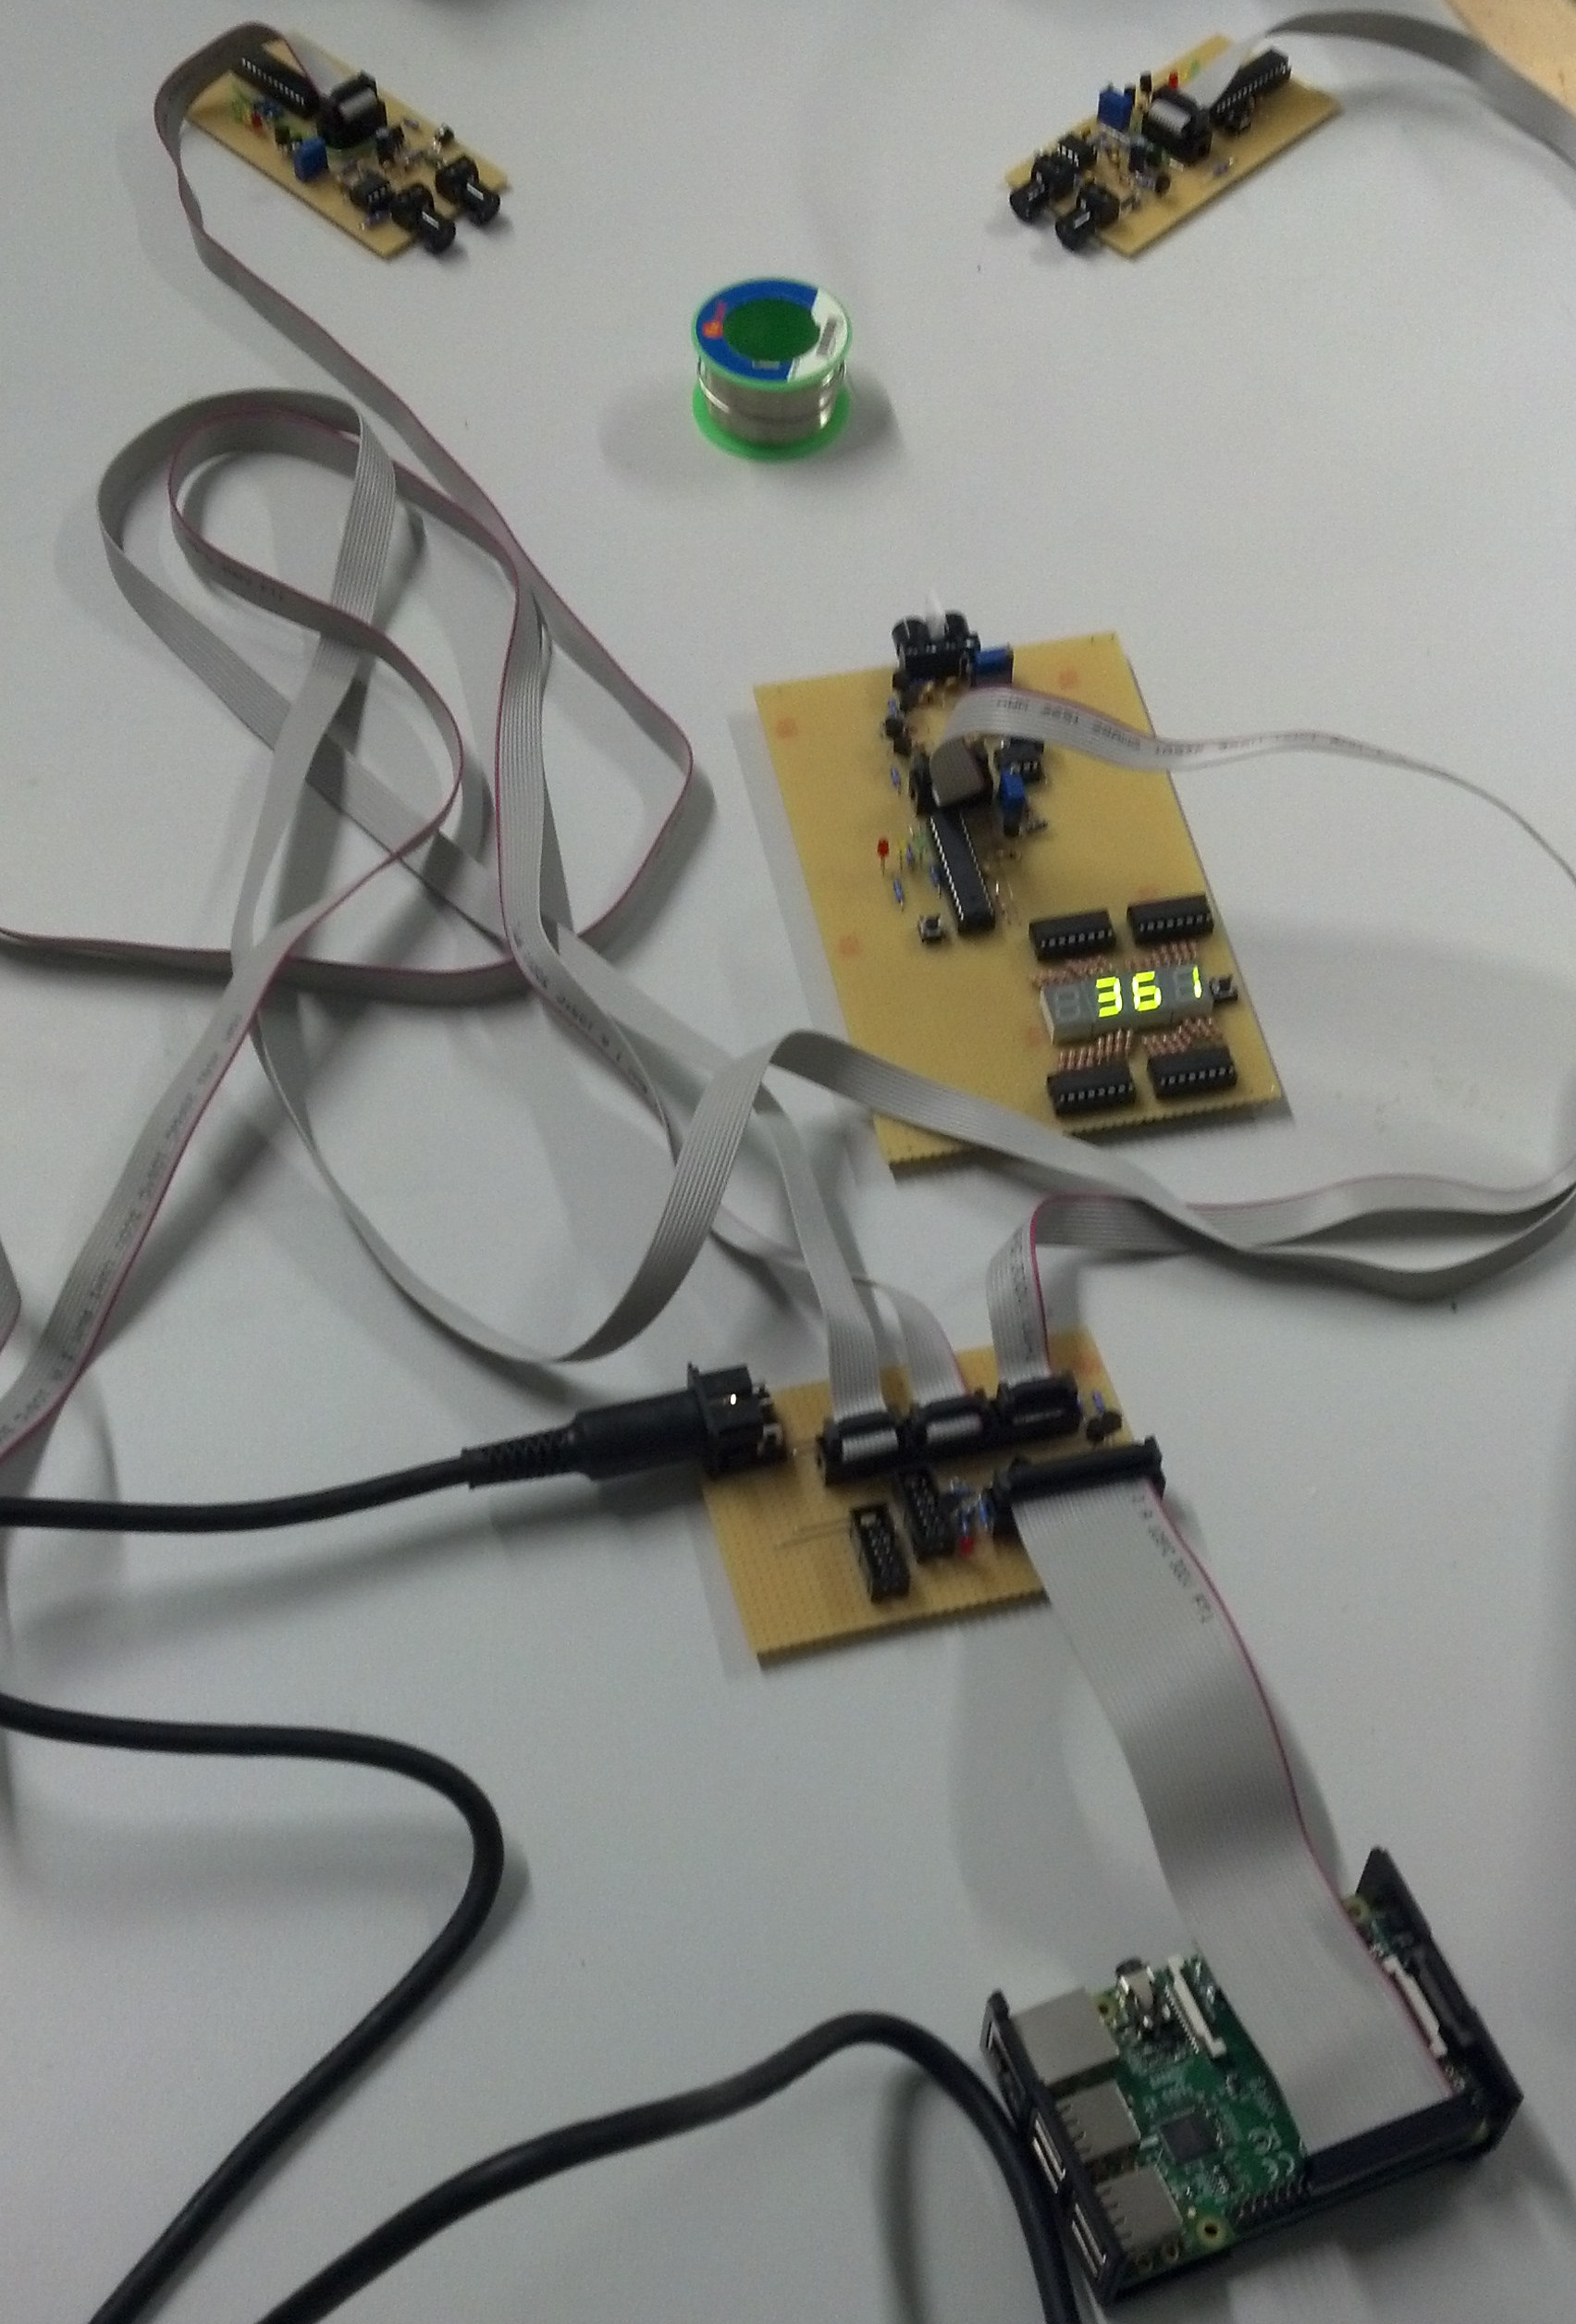
\includegraphics[width=(\textwidth), angle=0]{fotos/aufbau.jpg}
	\caption{Aufbau und Anordnung bei der Positionsbestimmung} \label{p:3}
\end{figure}
In der GUI können die Positionen der Sensoren bestimmt werden, damit eine exakte Positionsbestimmung relativ zu ihnen möglich ist.
	%!TEX root = ../dokumentation.tex

%\chapter{Schluss}



	% Anhang
	\clearpage
	\pagenumbering{roman}

	% Abbildungsverzeichnis
	\cleardoublepage
	\listoffigures

	%Tabellenverzeichnis
	\cleardoublepage
	\listoftables

	% Quellcodeverzeichnis
	\cleardoublepage
	\lstlistoflistings

	% Literaturverzeichnis
	\cleardoublepage
	\printbibliography

	% Abkürzungsverzeichnis
	\cleardoublepage
	\phantomsection \label{listofacs}
	\addcontentsline{toc}{chapter}{\langabkverz}
	%!TEX root = ../dokumentation.tex

\chapter*{\langabkverz}
%nur verwendete Akronyme werden letztlich im Dokument angezeigt
\begin{acronym}[YTMMM]
\setlength{\itemsep}{-\parsep}

\acro{AGPL}{Affero GNU General Public License}
\acro{PWM}{Pulsweitenmodulation}
\acro{CAD}{}
\acro{CERN}{Europäische Organisation für Kernforschung}
\acro{SPICE}{Simulation Program with Integrated Circuit Emphasis}
\acro{TWI}{Two Wire Interface: Serieller Multimaster-Bus über zwei Leitungen, auch I\textsuperscript{2}C genannt}
\acro{GUI}{Graphical User Interface, Grafische Benutzerschnittstelle}
\acro{LED}{Licht-emittierende Diode}
\acro{GPIO}{General-purpose input/output: Programmierbare digitale Ein- \& Ausgangspins}
\acro{HDMI}{High-Definition Multimedia Interface, digitale Schnittstelle z.B. für Bildschirme}
\acro{ISP}{In-System-Programming: Schnittstelle, mit der Mikrocontroller im eingebauten Zustand programmiert werden können}

\end{acronym}


	% Glossar
	\printglossary[style=altlist,title=\langglossar]
\end{document}
